%%%%%%%%%%%%%%%%%%%%%%%%%%%%%%%%%%%%%%%%%%%%%%%%%%%%%%%%%%%%%%%%%%%%%%%%%%%%%
%
%  System        : 
%  Module        : 
%  Object Name   : $RCSfile$
%  Revision      : $Revision$
%  Date          : $Date$
%  Author        : $Author$
%  Created By    : Robert Heller
%  Created       : Mon Apr 7 08:03:44 2025
%  Last Modified : <250522.1101>
%
%  Description 
%
%  Notes
%
%  History
% 
%%%%%%%%%%%%%%%%%%%%%%%%%%%%%%%%%%%%%%%%%%%%%%%%%%%%%%%%%%%%%%%%%%%%%%%%%%%%%
%
%    Copyright (C) 2025  Robert Heller D/B/A Deepwoods Software
%			51 Locke Hill Road
%			Wendell, MA 01379-9728
%
%    This program is free software; you can redistribute it and/or modify
%    it under the terms of the GNU General Public License as published by
%    the Free Software Foundation; either version 2 of the License, or
%    (at your option) any later version.
%
%    This program is distributed in the hope that it will be useful,
%    but WITHOUT ANY WARRANTY; without even the implied warranty of
%    MERCHANTABILITY or FITNESS FOR A PARTICULAR PURPOSE.  See the
%    GNU General Public License for more details.
%
%    You should have received a copy of the GNU General Public License
%    along with this program; if not, write to the Free Software
%    Foundation, Inc., 675 Mass Ave, Cambridge, MA 02139, USA.
%
% 
%
%%%%%%%%%%%%%%%%%%%%%%%%%%%%%%%%%%%%%%%%%%%%%%%%%%%%%%%%%%%%%%%%%%%%%%%%%%%%%

\documentclass[letterpaper,twoside,12pt]{article}
\usepackage{graphicx}
\usepackage{mathptm}
\usepackage{times}
\PassOptionsToPackage{hyphens}{url}
\usepackage{ifpdf}
\ifpdf
\usepackage[pdftex,
            pagebackref=true,
            colorlinks=true,
            linkcolor=blue,
            unicode
           ]{hyperref}
\else
\usepackage[ps2pdf,
            pagebackref=true,
            colorlinks=true,
            linkcolor=blue,
            unicode
           ]{hyperref}
\usepackage{pspicture}
\fi
\pagestyle{headings}
\usepackage{listings}
\lstset{language=Python,basicstyle=\footnotesize}
\emergencystretch=50pt
\setcounter{tocdepth}{3}
\setcounter{secnumdepth}{3}
\title{Gemma M0 Embroidery}
\author{Robert Heller}
\date{\today}

\begin{document}

\maketitle

\tableofcontents

\part{Introduction}
\section{Who I am}

My name is Robert Heller.  I have been writing computer programs for over 50
years.

\section{What we will be making}

We will be creating a light up embroidery piece.  We will use a small, 
sew-able microprocessor with some sew-able lighting devices.

\part{Materials and Tools}

We will be using various materials and tools to make this project.  Some of 
the materials and tools might be materials and tools you are familiar with and 
some might be new.

\section{The electronics}

We will be using some electronic components in this project.  The main 
components are self contained small circuit boards with sew-able pads around 
the edges.  These circuit boards are designed to be sewn onto fabric, not 
unlike sewing on a decorative button.

\subsection{The microprocessor: Gemma M0}

\begin{figure}[hbpt]\begin{centering}%
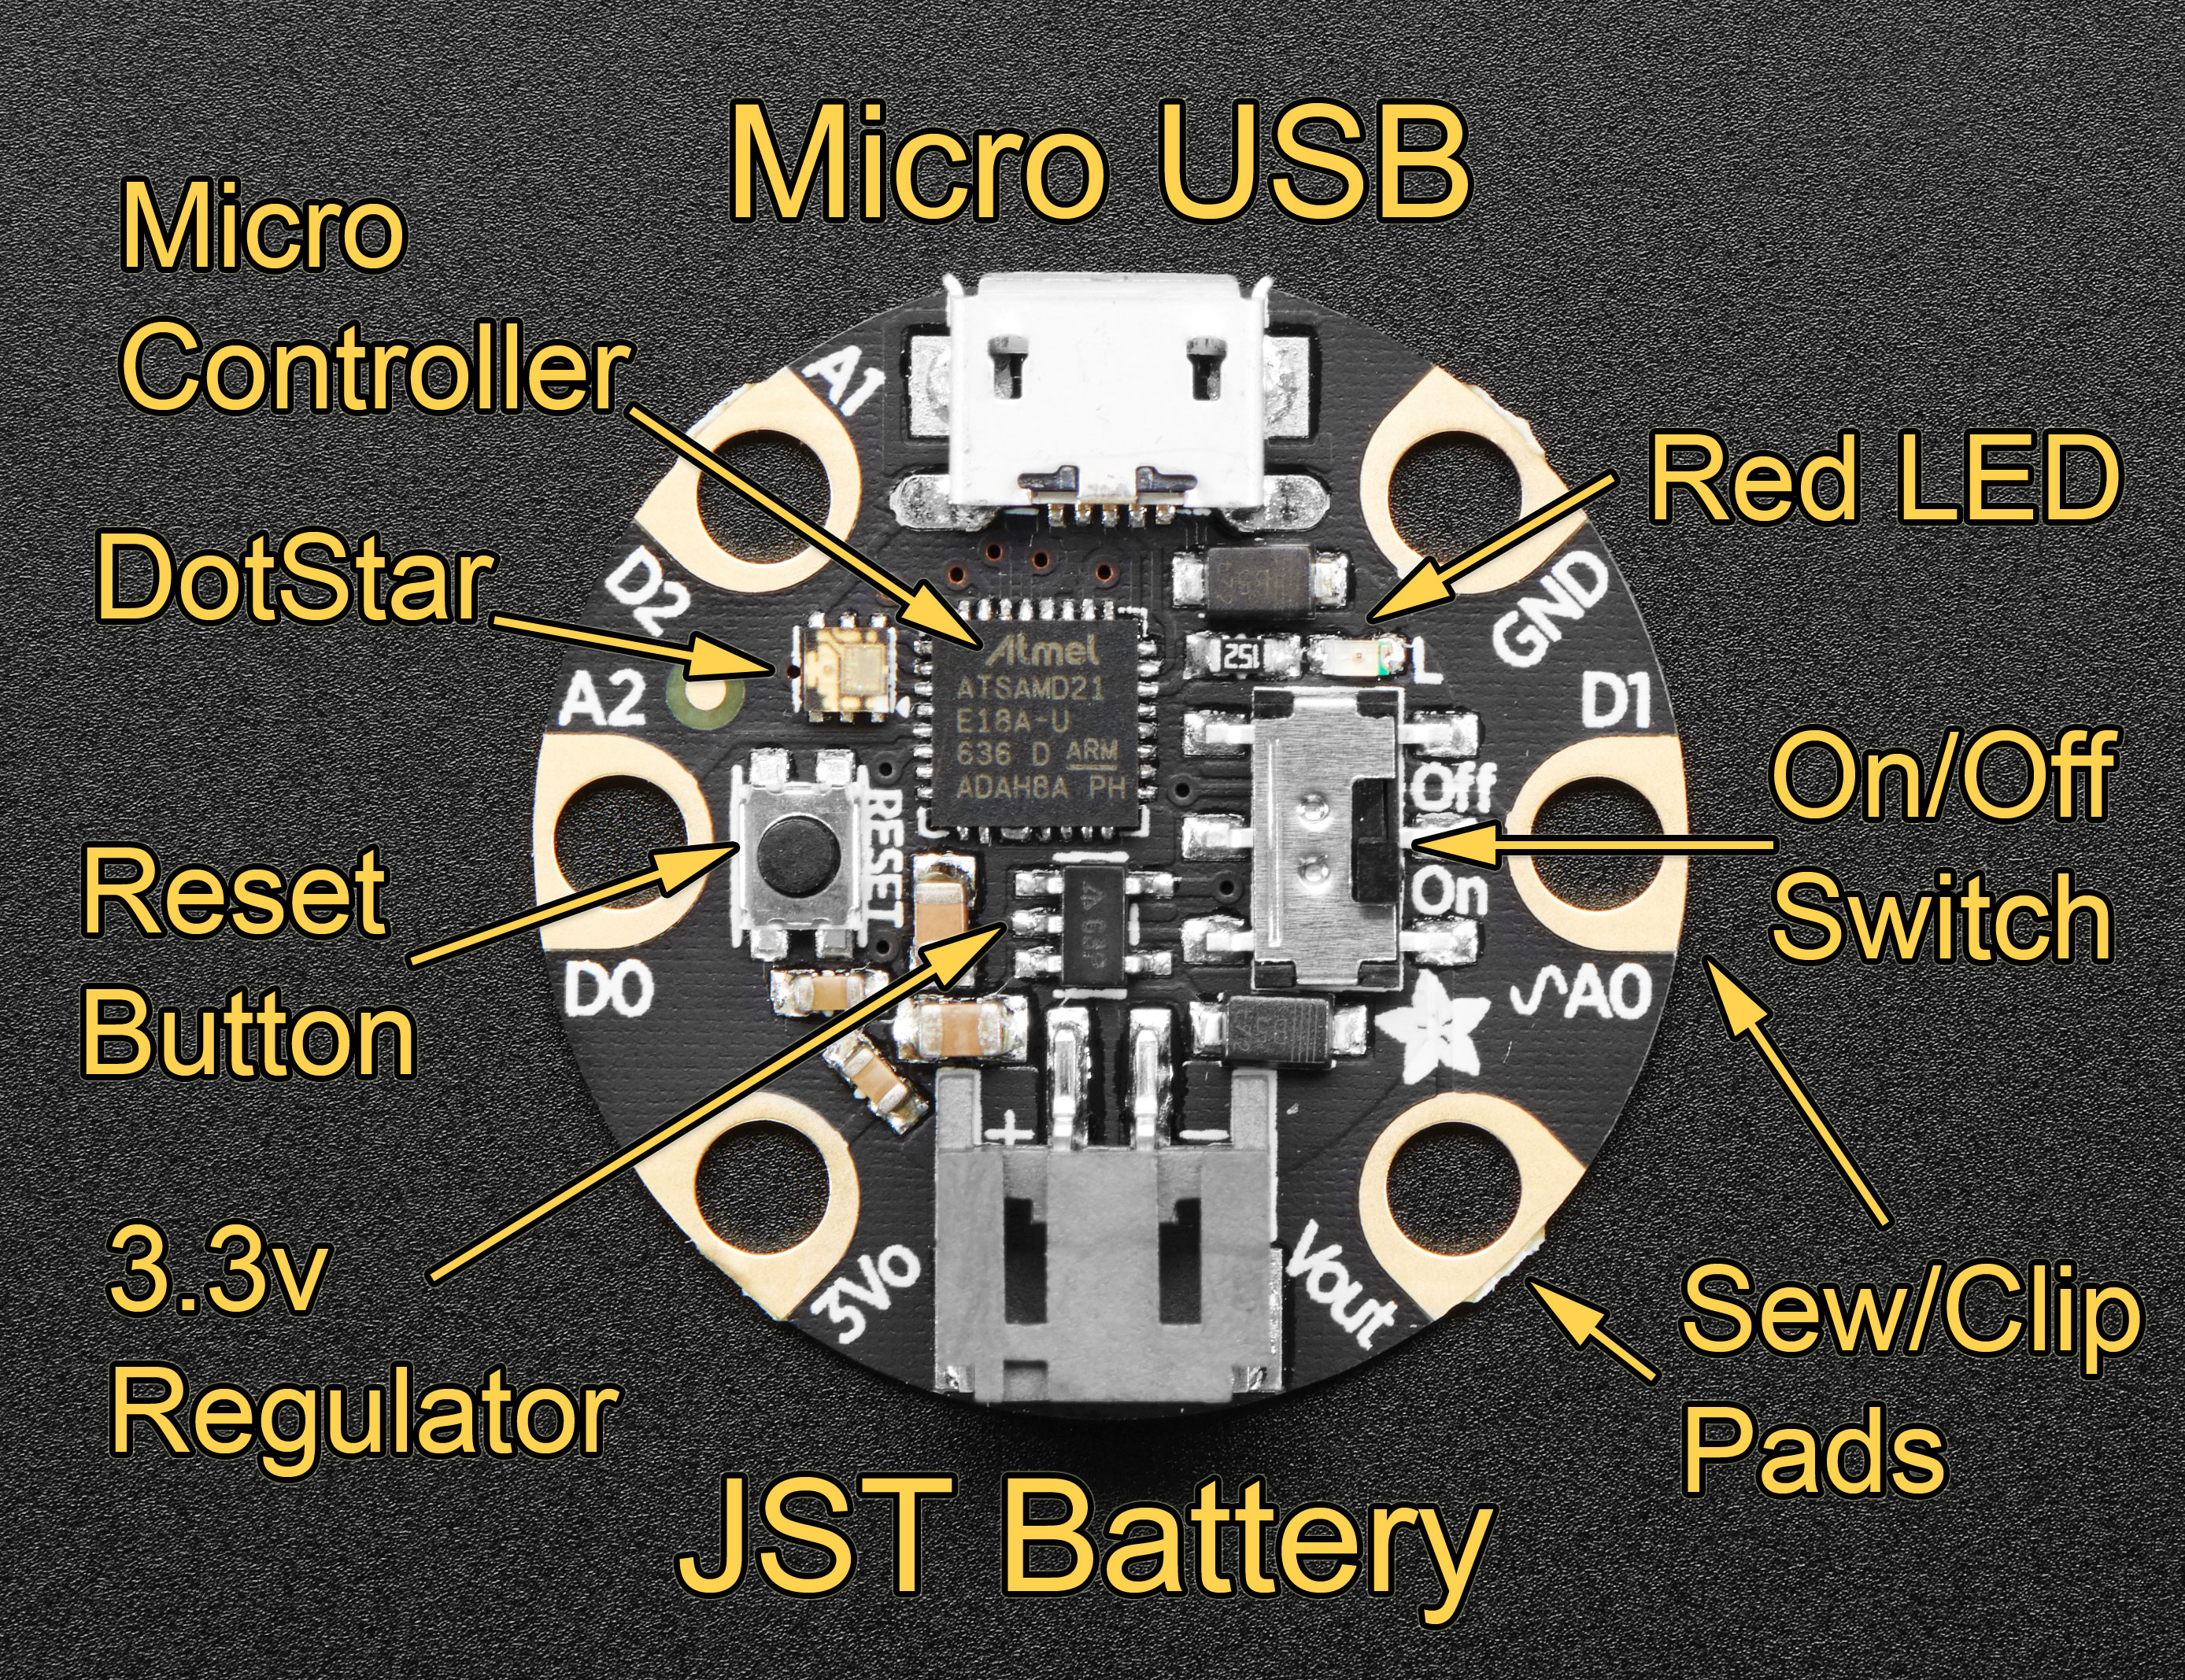
\includegraphics[width=5in]{gemma_guide.png}
\caption{Gemma M0 Main features}
\label{fig:gemmaguide}
\end{centering}\end{figure}
\begin{figure}[hbpt]\begin{centering}%
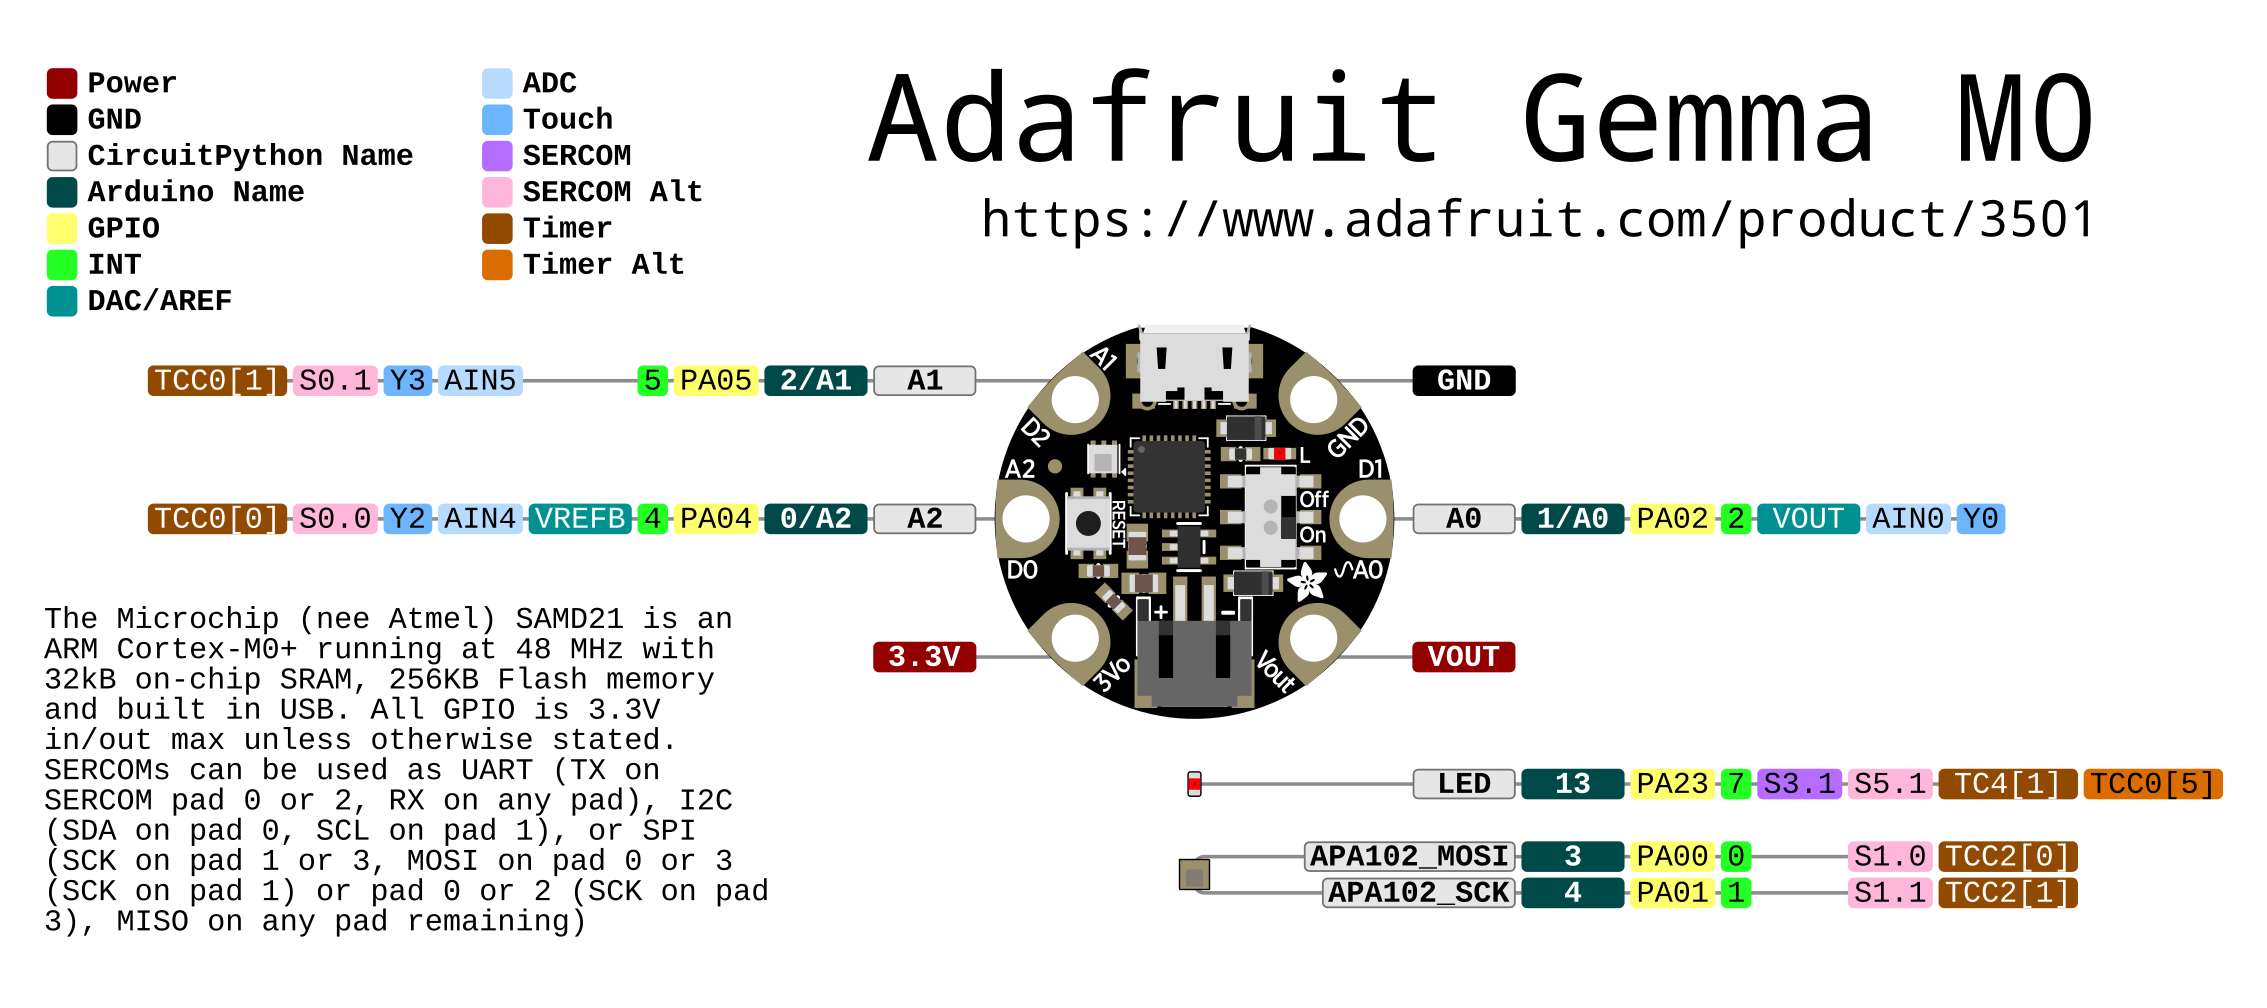
\includegraphics[width=5in]{adafruit_gemma_Adafruit_GEMMA_M0_pinout.png}
\caption{Gemma M0 pin-out}
\label{fig:gemmapinout}
\end{centering}\end{figure}
We will be using the Adafruit Gemma M0 as the main processing element\footnote{
\url{https://www.adafruit.com/product/3501}.} processor board, shown in
Figures~\ref{fig:gemmaguide} and \ref{fig:gemmapinout}. This small board
features a powerful 32-bit ARM Cortex M0 processor. It is preloaded with
CircuitPython\footnote{A small Python system meant for embedded processors.} 
and we will be writing a small program in Python to bring our project to life.
\clearpage
\subsection{The NeoPixel}
\begin{figure}[hbpt]\begin{centering}%
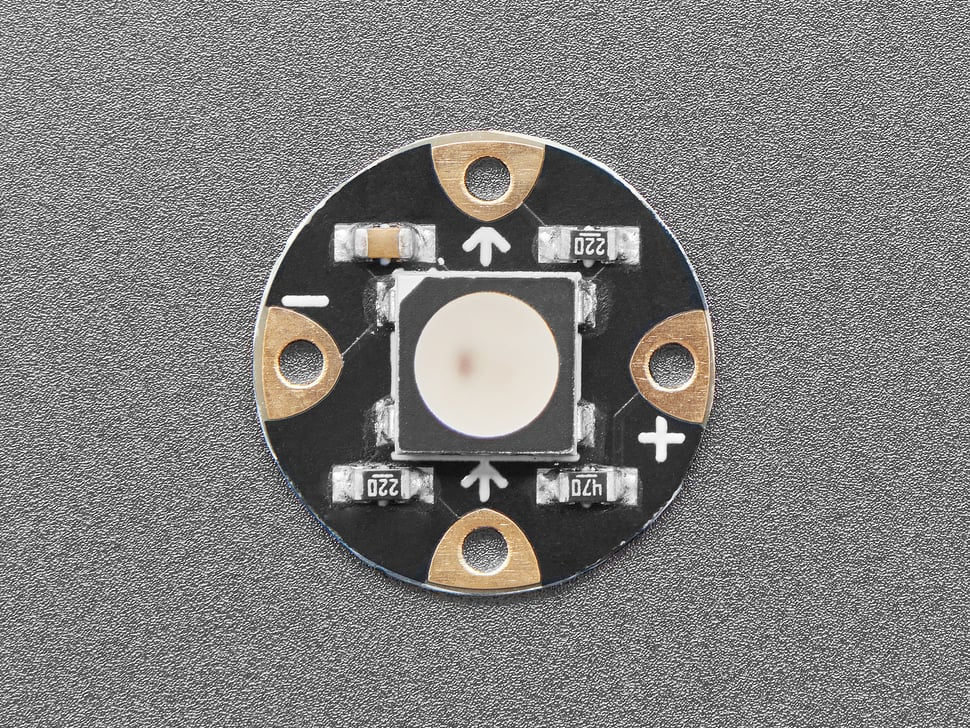
\includegraphics[width=5in]{FloraNeoPixel.png}
\caption{Flora NeoPixel}
\label{fig:floraneopixel}
\end{centering}\end{figure}
We will be using Flora
NeoPixels\footnote{\url{https://www.adafruit.com/product/1260}.} to add lit up
elements to our embroidery project, show in Figure~\ref{fig:floraneopixel}.
These small sew-able circuit boards feature an addressable full color LED light
capable of over 16 million possible colors.  Under program control the light 
can change color, blink, and change brightness level.
\clearpage
\subsection{Snaps}
\begin{figure}[hbpt]\begin{centering}%
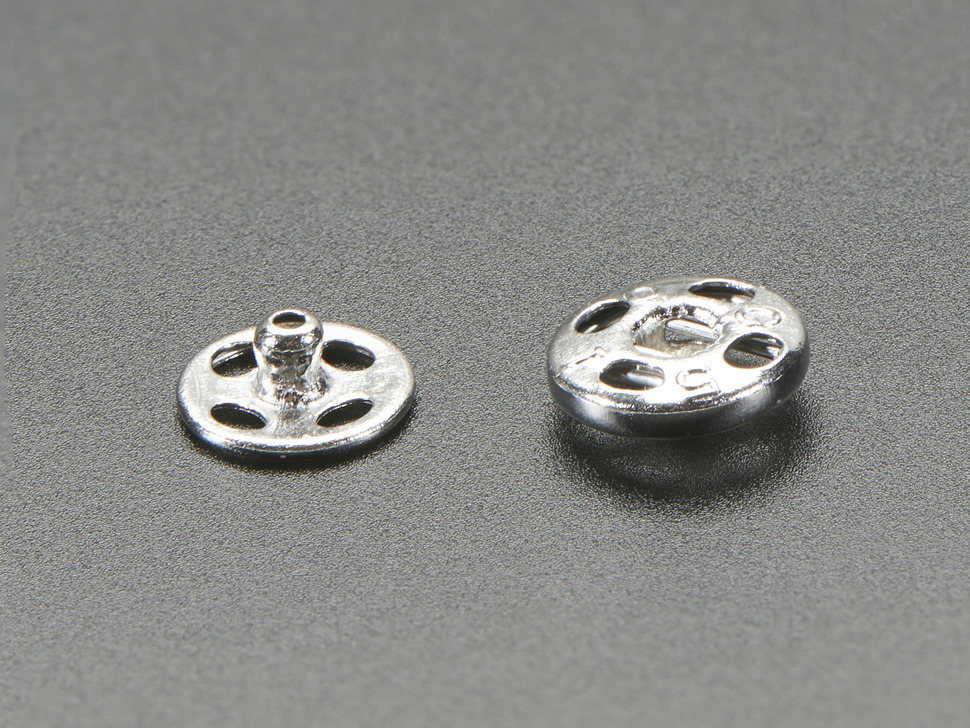
\includegraphics[width=5in]{snap.png}
\caption{Small Metal Snaps}
\label{fig:snaps}
\end{centering}\end{figure}
We will be using a small metal snap, shown in Figure~\ref{fig:snaps}, as a 
switch.  This will be used to select between two operating modes, such as
different colors or blink patterns.
\clearpage
\subsection{Conductive Thread}
\begin{figure}[hbpt]\begin{centering}%
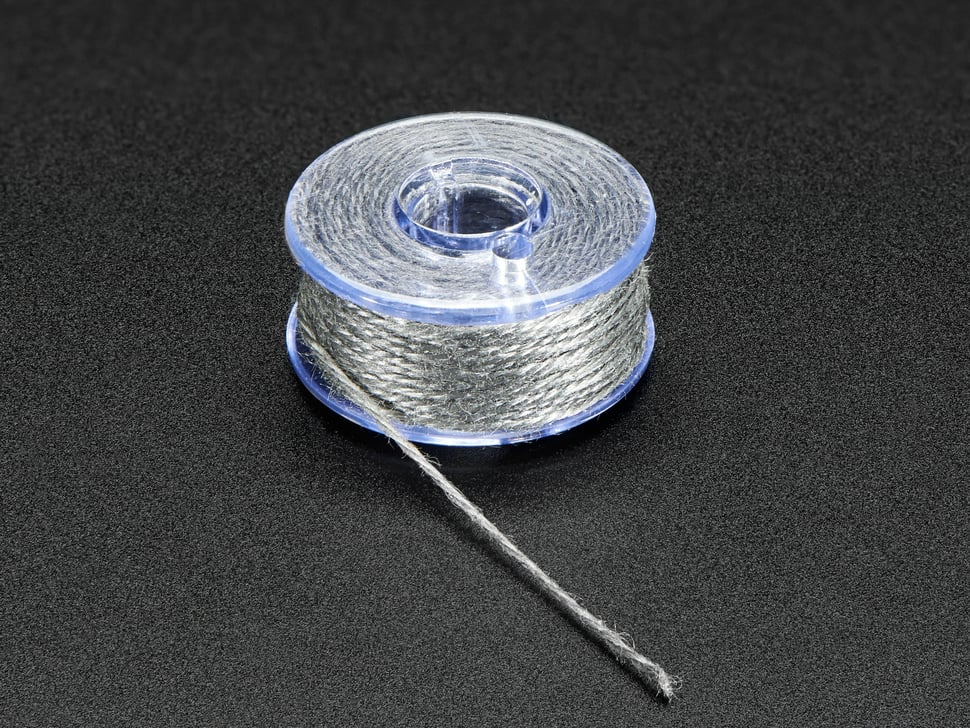
\includegraphics[width=5in]{conductivethread.png}
\caption{Conductive Thread}
\label{fig:conductivethread}
\end{centering}\end{figure}
We will be using stainless steel thread, show in 
Figure~\ref{fig:conductivethread}, to provide the electrical circuits between 
the various components. 
\clearpage
\subsection{Battery Holder and extension cable}
\begin{figure}[hbpt]\begin{centering}%
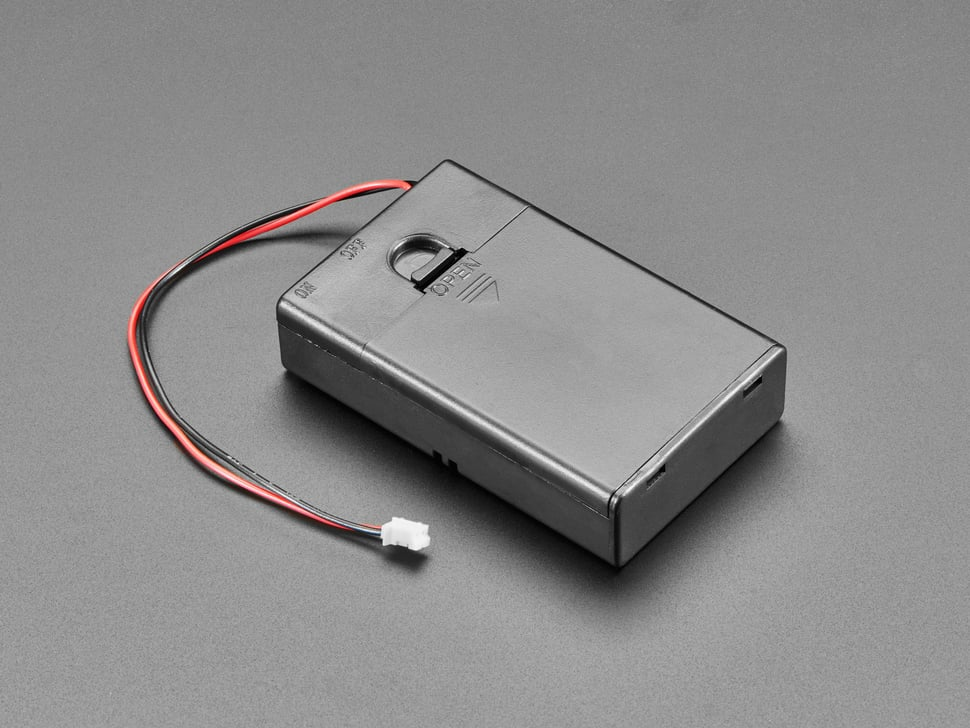
\includegraphics[width=5in]{BatteryHolder.png}
\caption{Battery Holder}
\label{fig:batteryholder}
\end{centering}\end{figure}
\begin{figure}[hbpt]\begin{centering}%
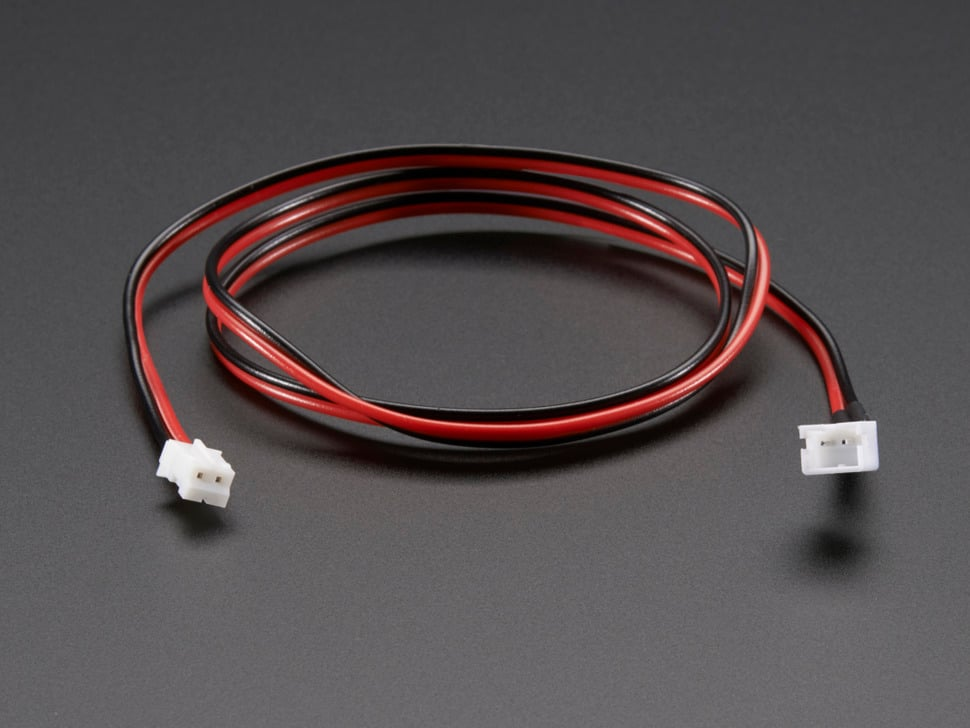
\includegraphics[width=5in]{ExtenssionCable.png}
\caption{Extension Cable}
\label{fig:extenssioncable}
\end{centering}\end{figure}
We will be powering the circuit with AAA batteries in a battery holder, shown 
in Figure~\ref{fig:batteryholder} and use an extension cable, shown in 
Figure~\ref{fig:extenssioncable} to allow some flexibility in the placement of 
the battery holder.
\clearpage
\subsection{USB Cable}
\begin{figure}[hbpt]\begin{centering}%
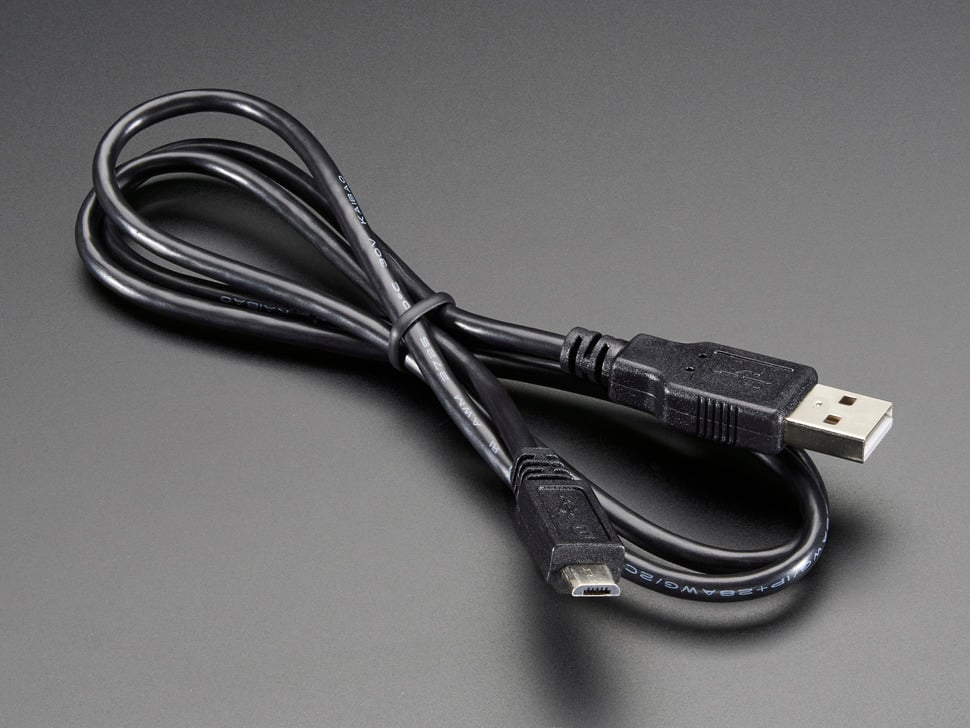
\includegraphics[width=5in]{USBCable.png}
\caption{USB Cable}
\label{fig:usbcable}
\end{centering}\end{figure}
Finally, we will use a USB Cable, shown in Figure~\ref{fig:usbcable} to 
program the micro-controller.
\section{Other materials}
In addition to the electronic components, we will be using some conventional 
embroidery and sewing materials.
\clearpage
\subsection{Embroidery Thread}
\begin{figure}[hbpt]\begin{centering}%
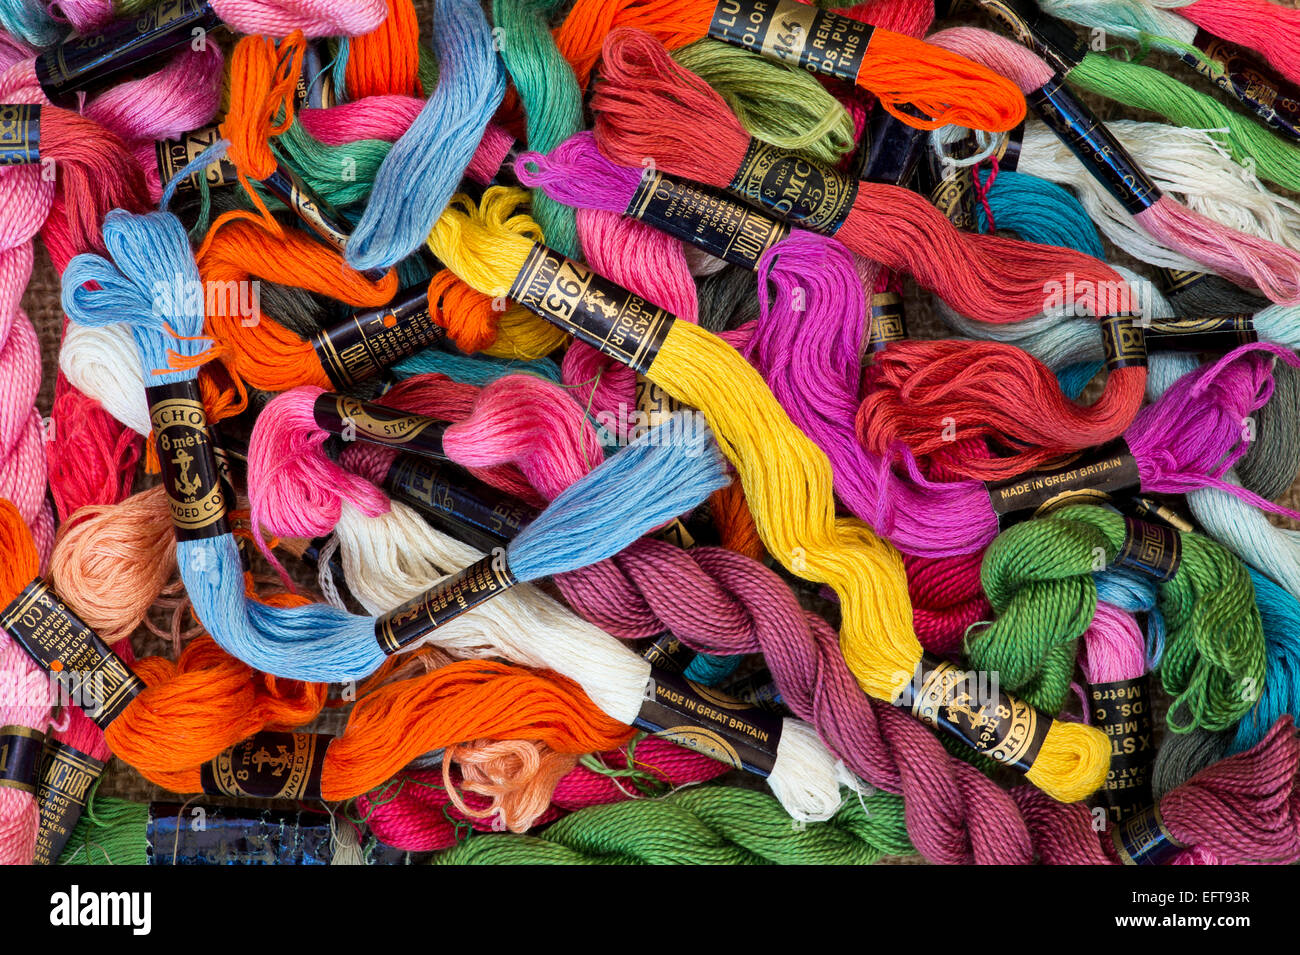
\includegraphics[width=5in]{embroiderythreads.png}
\caption{Embroidery Threads}
\label{fig:embroiderythreads}
\end{centering}\end{figure}
For the bulk of the embroidery design will be be using standard embroidery 
thread.
\clearpage
\subsection{Fabric Scraps}
\begin{figure}[hbpt]\begin{centering}%
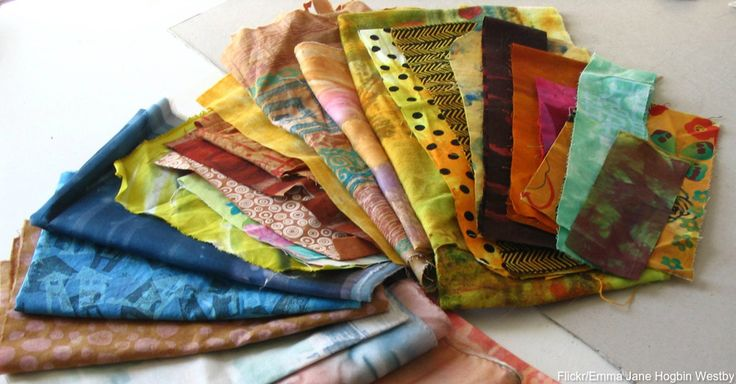
\includegraphics[width=5in]{FabricScraps.png}
\caption{Fabric Scraps}
\label{fig:fabricscraps}
\end{centering}\end{figure}
For the snap switch and possibly to make a pocket or pouch for the battery 
holder will be be using pieces of scrap fabric.
\clearpage
\subsection{Clear Nail Polish}
\begin{figure}[hbpt]\begin{centering}%

\includegraphics[width=5in]{ClearNailPolish.png}
\caption{Clear Nail Polish}
\label{fig:clearnailpolish}
\end{centering}\end{figure}
The conductive thread is too springy to hold knots, so we will use clear nail 
polish to secure the knots we will be making with the conductive thread.
\clearpage
\section{The Tools}
We will be use some basic sewing tools.
\subsection{Needles}
\begin{figure}[hbpt]\begin{centering}%
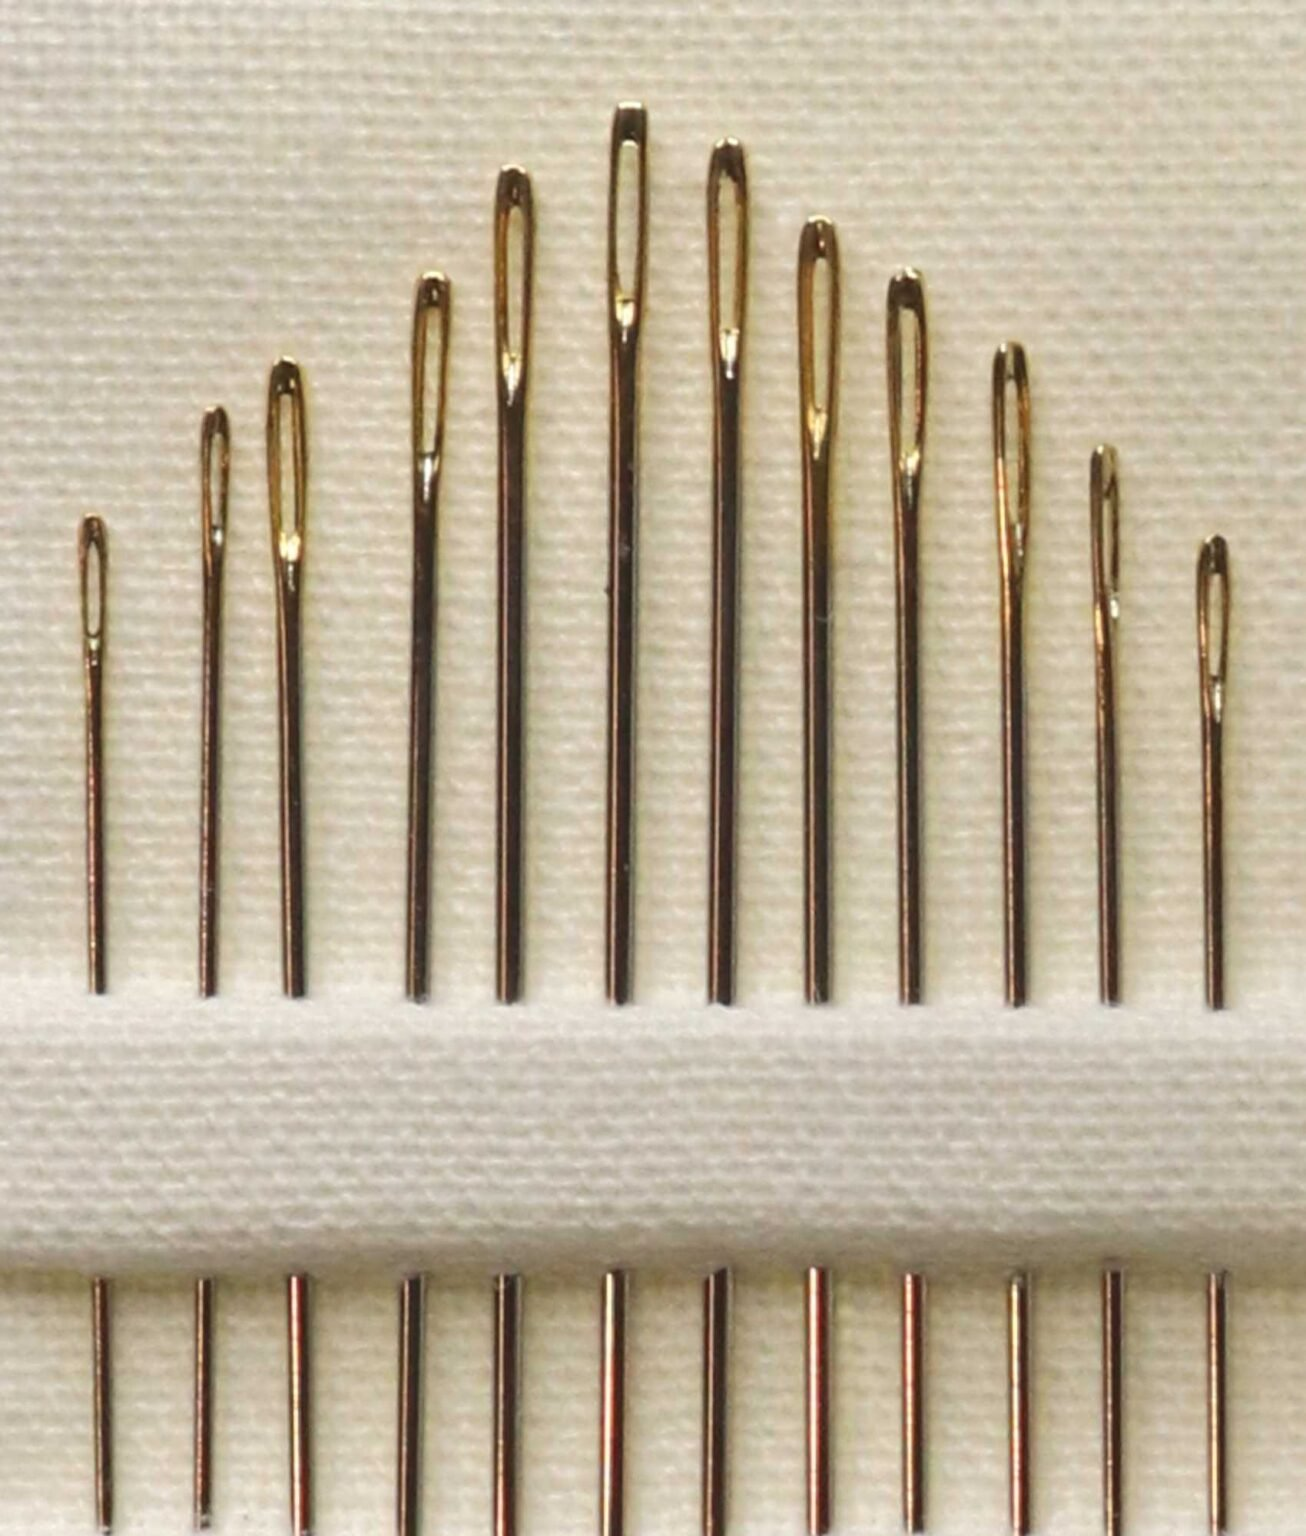
\includegraphics[width=5in]{Needles.png}
\caption{Needles}
\label{fig:needles}
\end{centering}\end{figure}
Sewing needles, shown in Figure~\ref{fig:needles}.
\clearpage
\subsection{Scissors}
\begin{figure}[hbpt]\begin{centering}%
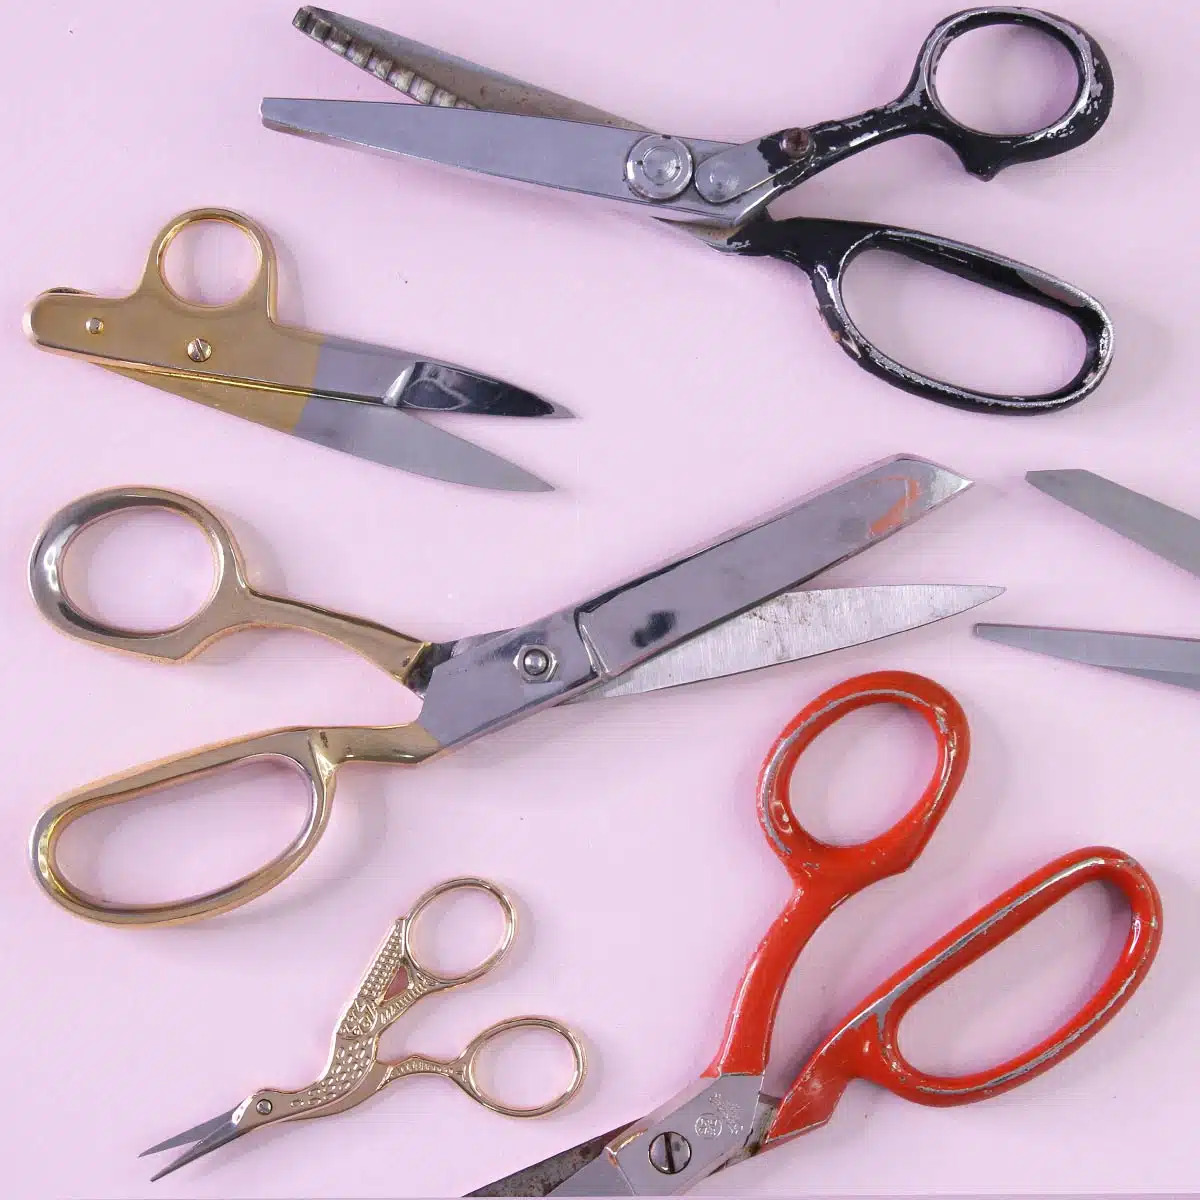
\includegraphics[width=5in]{Scissors.png}
\caption{Scissors}
\label{fig:scissors}
\end{centering}\end{figure}
Sewing scissors, shown in Figure~\ref{fig:scissors}.
\clearpage
\subsection{Embroidery hoop}
\begin{figure}[hbpt]\begin{centering}%
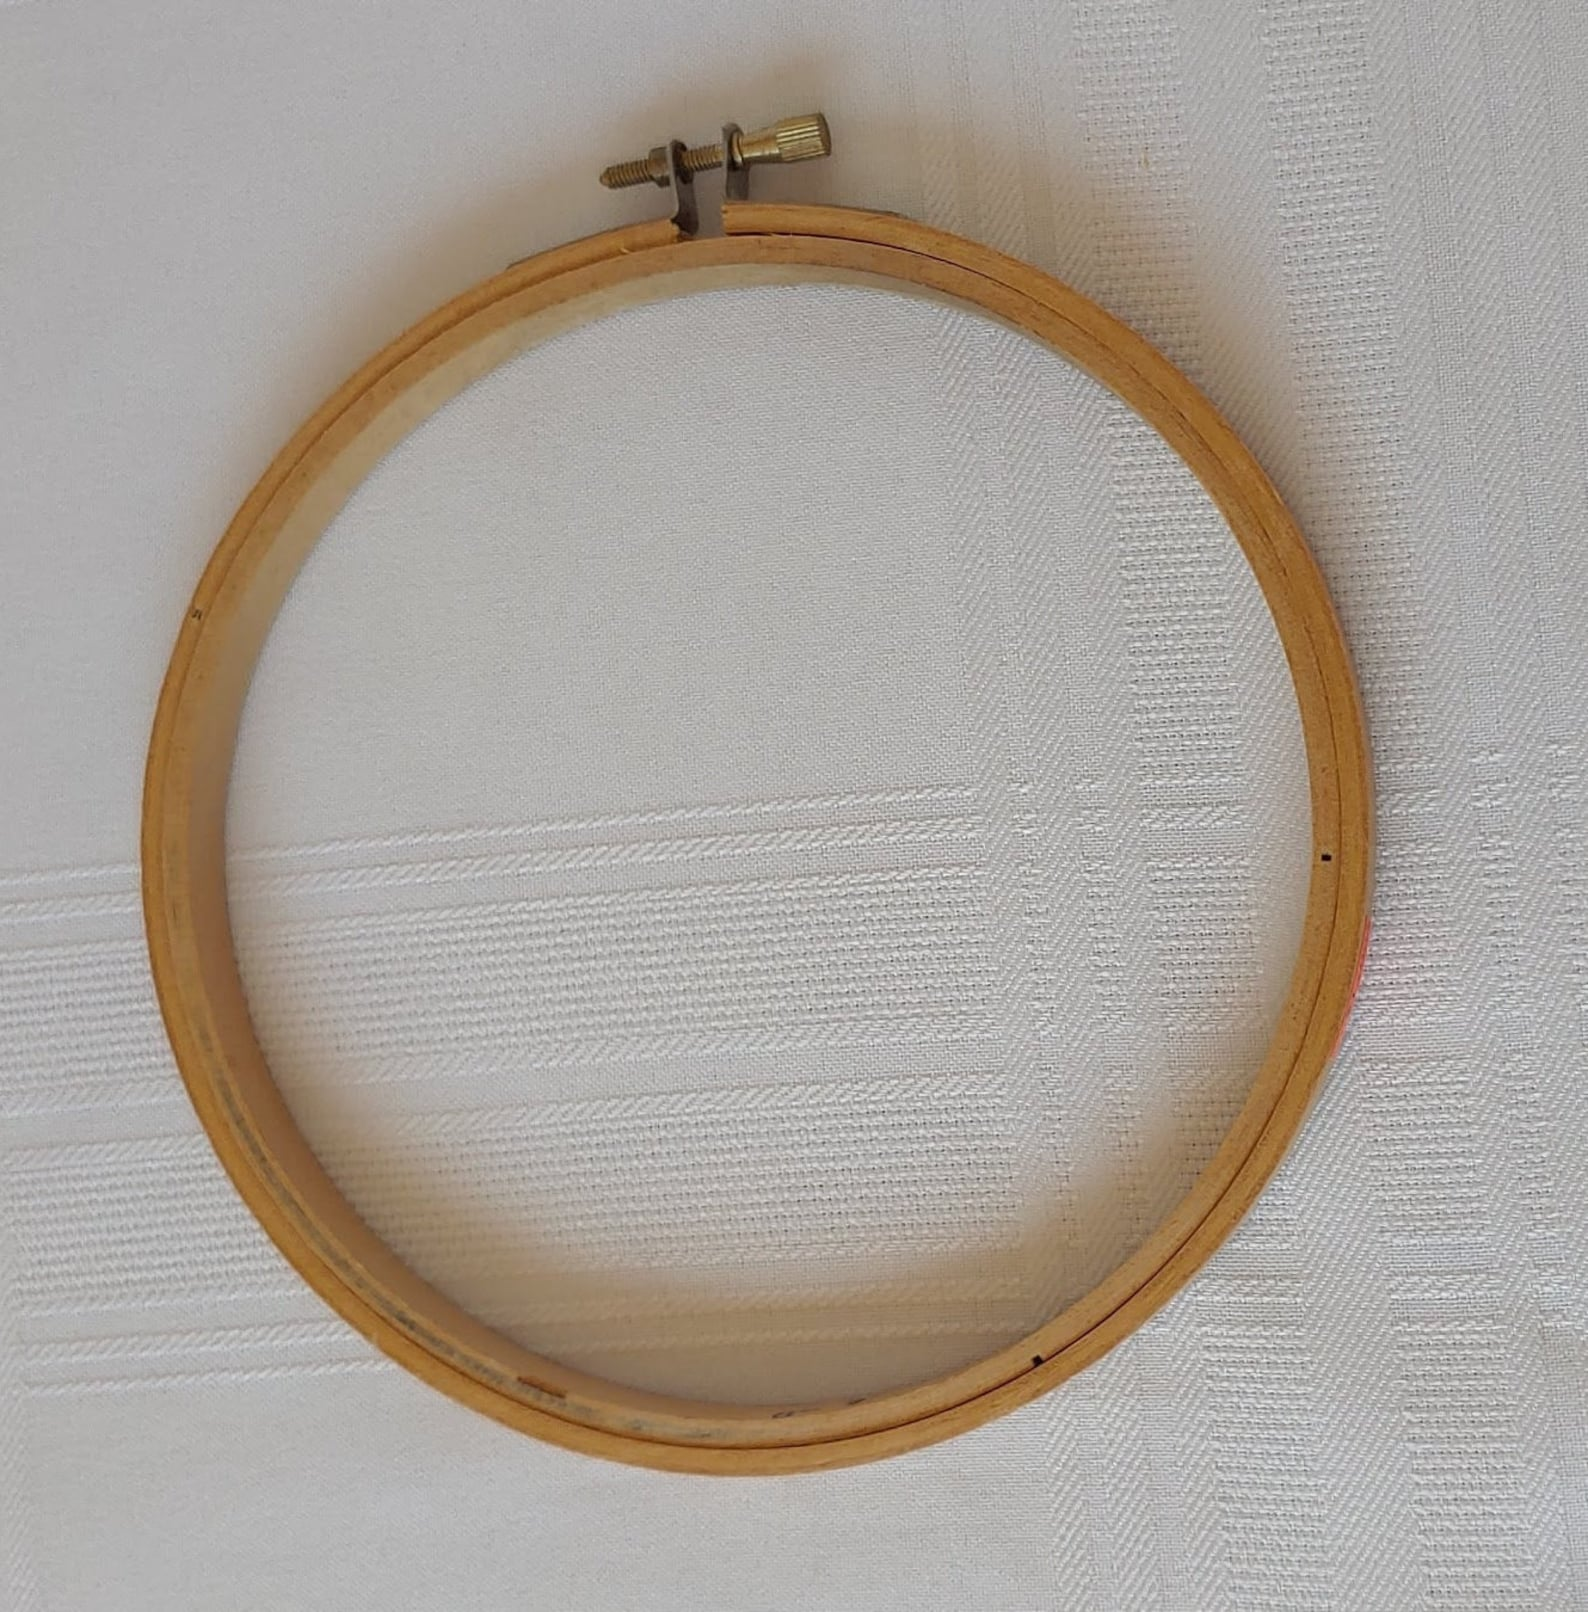
\includegraphics[width=5in]{Embroideryhoop.png}
\caption{Embroidery Hoop}
\label{fig:embroideryhoop}
\end{centering}\end{figure}
Embroidery hoop, shown in Figure~\ref{fig:embroideryhoop}.
\clearpage
\subsection{Fabric markers and tailor's chalk}
\begin{figure}[hbpt]\begin{centering}%
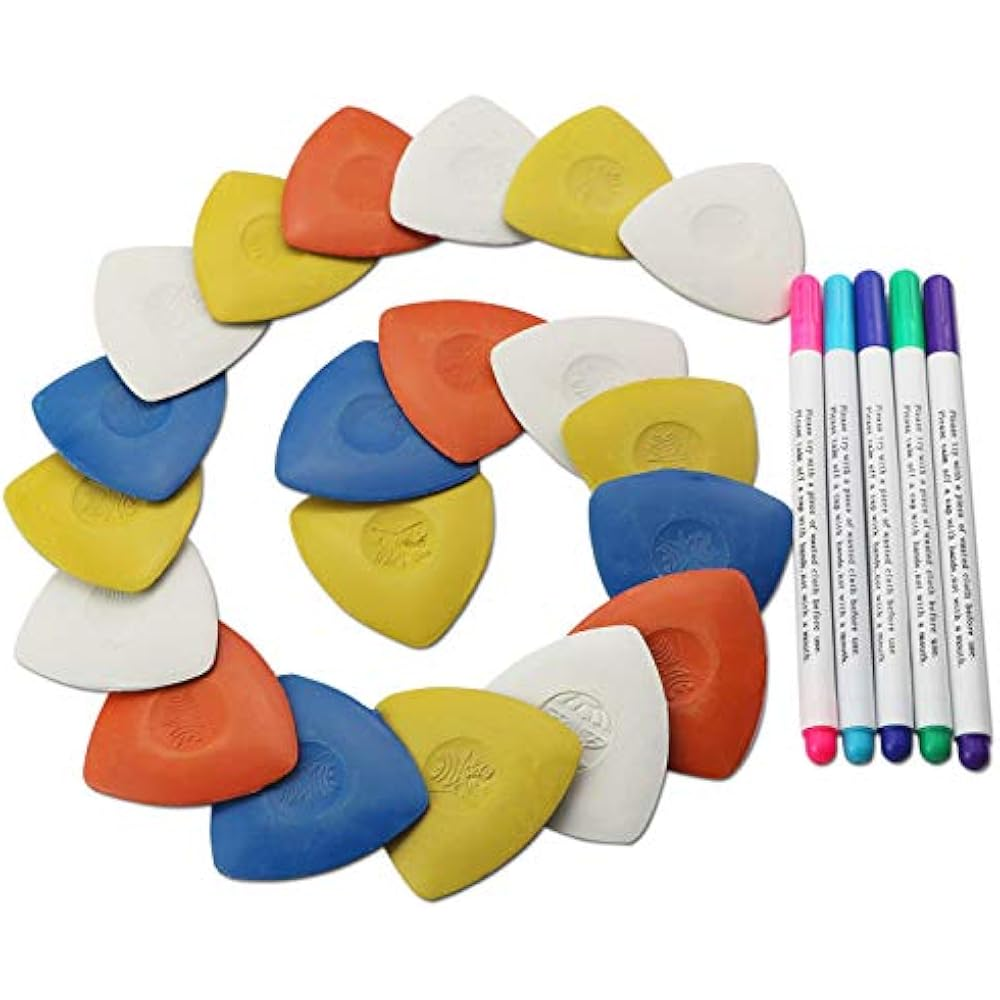
\includegraphics[width=5in]{Fabricmarkerstailorschalk.png}
\caption{Fabric Markers and Tailor's Chalk}
\label{fig:fabricmarkerstailorschalk}
\end{centering}\end{figure}
Fabric markers and tailor's chalk, shown in Figure~\ref{fig:fabricmarkerstailorschalk}.
\subsection{Paper and pencils}
\begin{figure}[hbpt]\begin{centering}%

\includegraphics[width=5in]{Paperandpencils.png}
\caption{Paper and Pencils}
\label{fig:paperandpencils}
\end{centering}\end{figure}
Paper and pencils, shown in Figure~\ref{fig:paperandpencils}.
\clearpage
\part{Designing the Embroidery}
Since we will be including a feature of the embroidery design lighting, it 
might make sense to include design elements that include lighting.  Here are 
some images of things that naturally ``light up''. 
\begin{figure}[hbpt]\begin{centering}%
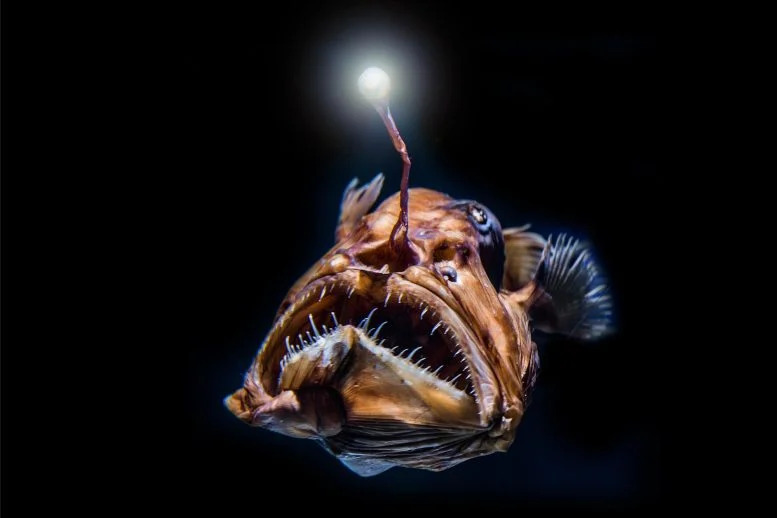
\includegraphics[height=2.25in]{Bioluminescence-Deep-Sea-Fish-777x518.png}
\caption{Bioluminescence Deep Sea Fish}
\label{fig:biolumfish}
\end{centering}\end{figure}
\begin{figure}[hbpt]\begin{centering}%
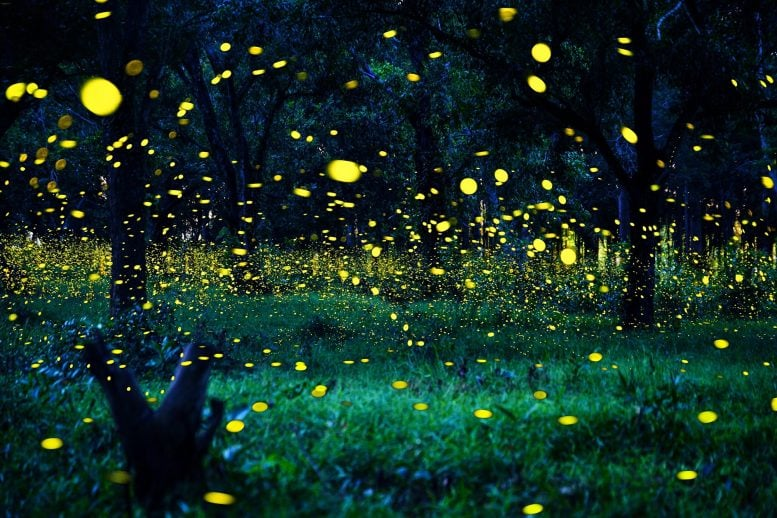
\includegraphics[height=2.25in]{Bioluminescence-Fireflies-777x518.png}
\caption{Bioluminescence Fireflies}
\label{fig:biolumflies}
\end{centering}\end{figure}
\clearpage 
\begin{figure}[hbpt]\begin{centering}%
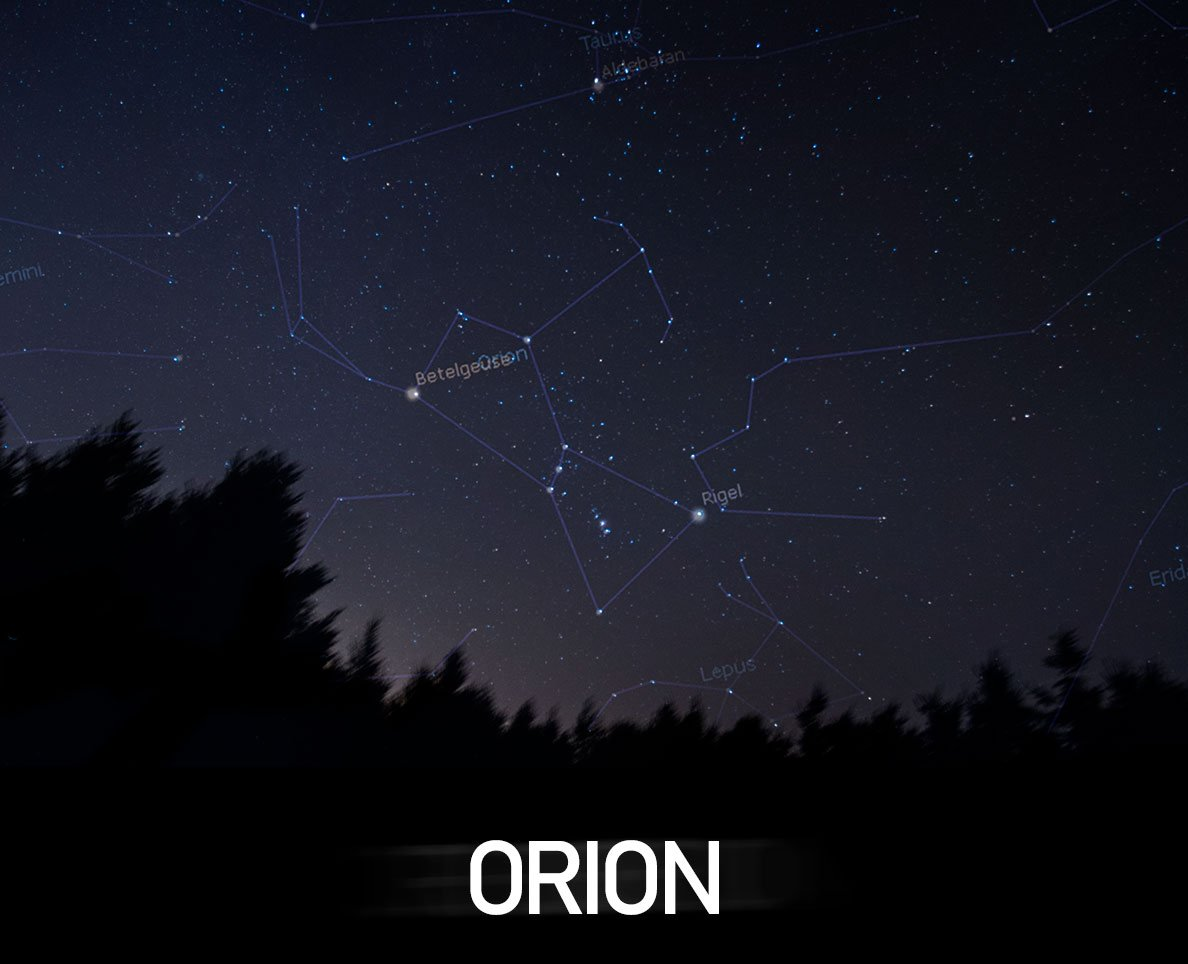
\includegraphics[height=2.25in]{orion.png}
\caption{Orion}
\label{fig:orion}
\end{centering}\end{figure}
\begin{figure}[hbpt]\begin{centering}%
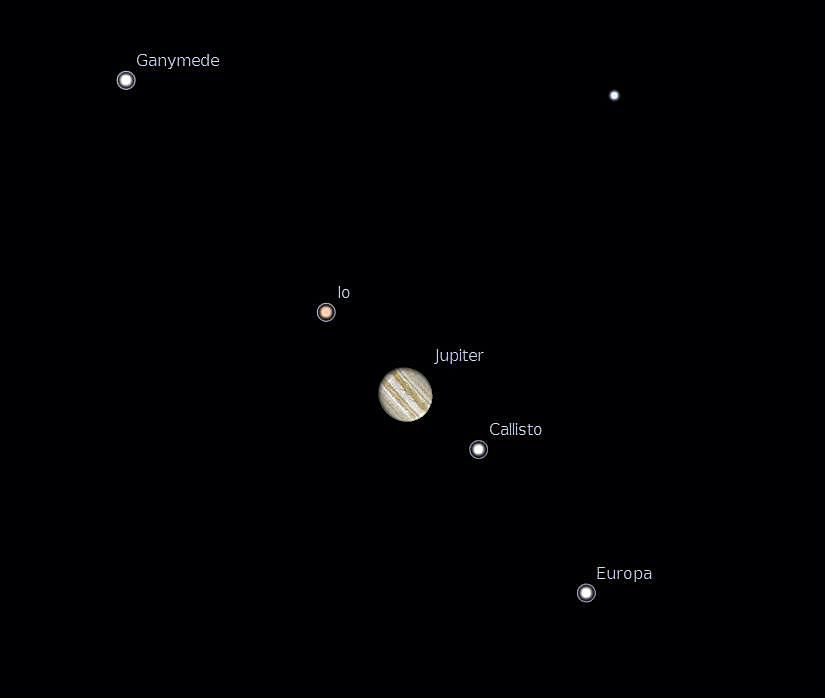
\includegraphics[height=2.25in]{Jupiter-and-moons-58b82f8c3df78c060e64eb8b.png}
\caption{Jupiter and Moons}
\label{fig:jupiterandmoons}
\end{centering}\end{figure}
\clearpage
\begin{figure}[hbpt]\begin{centering}%
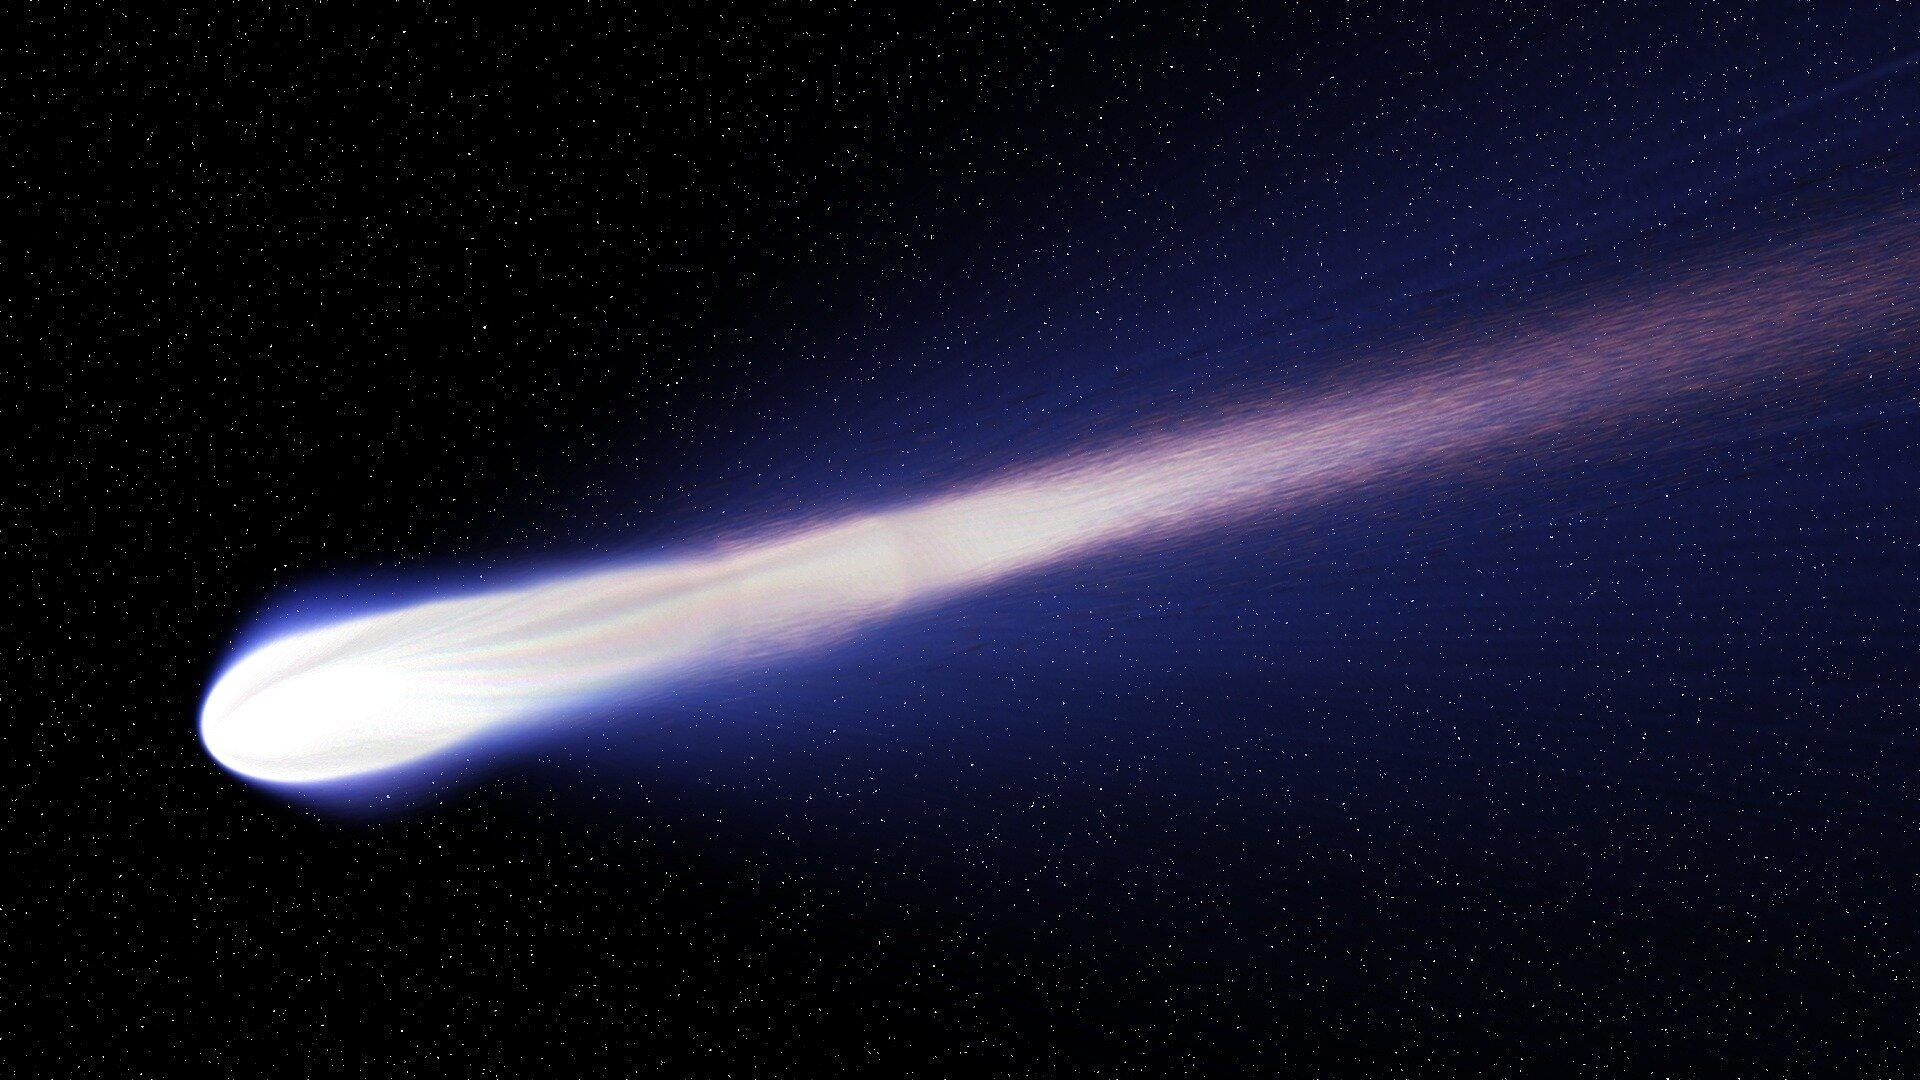
\includegraphics[height=2.25in]{comet.png}
\caption{Comet}
\label{fig:comet}
\end{centering}\end{figure}
\begin{figure}[hbpt]\begin{centering}%
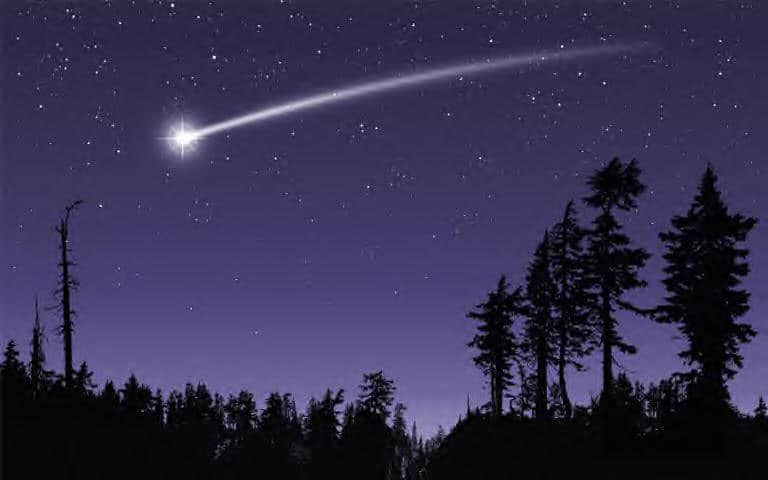
\includegraphics[height=2.25in]{shooting-star-1756306537.png}
\caption{Shooting Star}
\label{fig:shootingstar}
\end{centering}\end{figure}
\clearpage
\begin{figure}[hbpt]\begin{centering}%
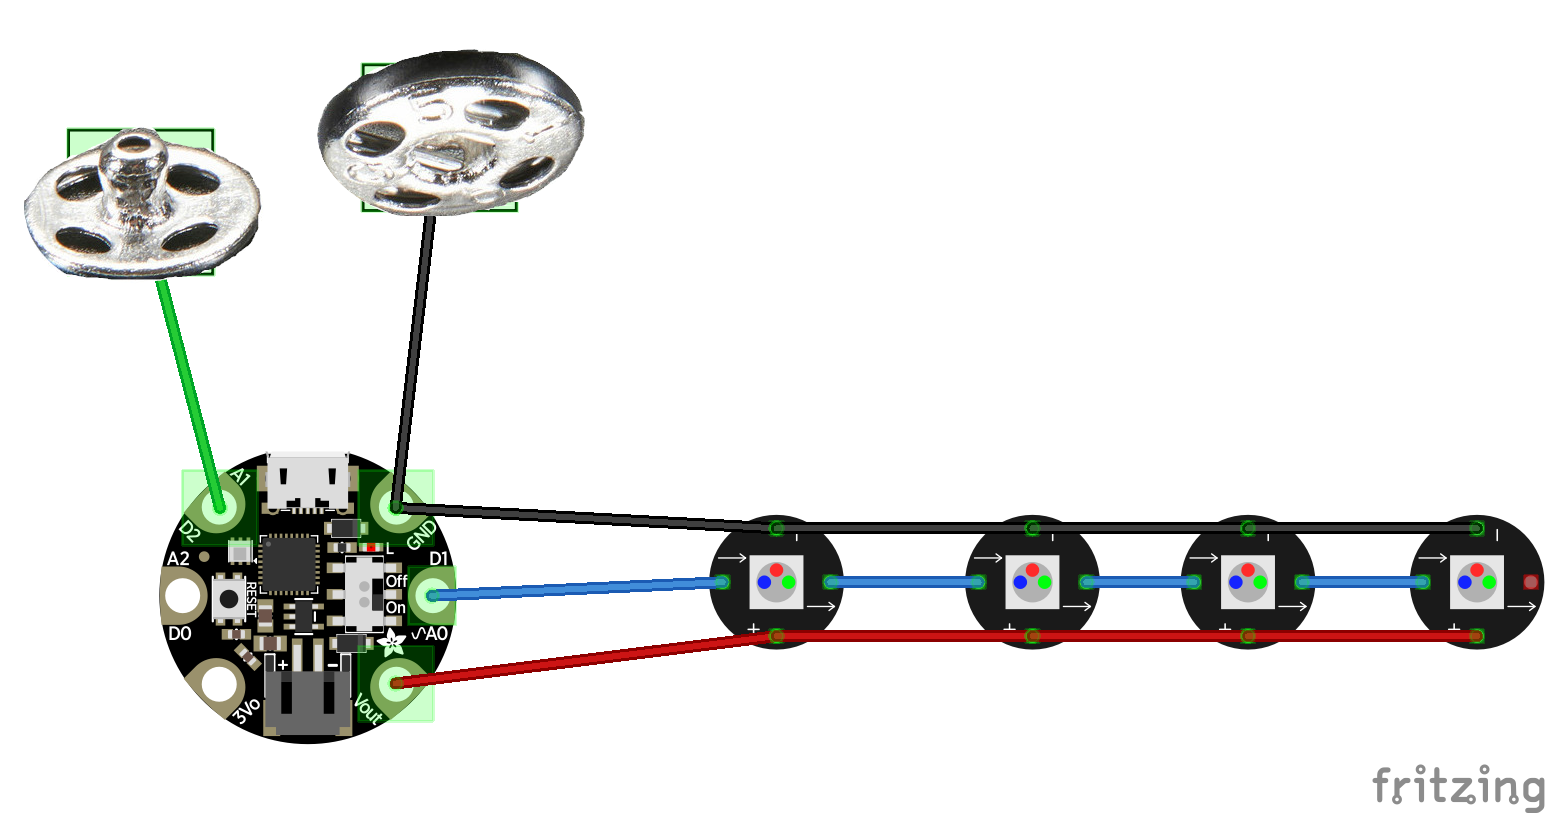
\includegraphics[width=4in]{CircuitDiagram_bb.png}
\caption{Circuit Diagram}
\label{fig:circuitdiagrame}
\end{centering}\end{figure}
And you need to also allow for the components of the circuit to be somewhere 
in the design.
\part{Sewing with conductive thread}
\section{''Wiring'' the circuit with conductive thread}
Wiring the circuit with conductive thread, is pretty straight forward.  Mostly 
just sewing with running stitches.  There are a couple of issues though.  The 
conductive thread is actually stainless steel and does not take to being 
knotted very well.  Also, one must be careful to avoid crossing circuit paths, 
which would cause short circuits.
\subsection{Installing the Embroidery Hoop}
\begin{figure}[hbpt]\begin{centering}%
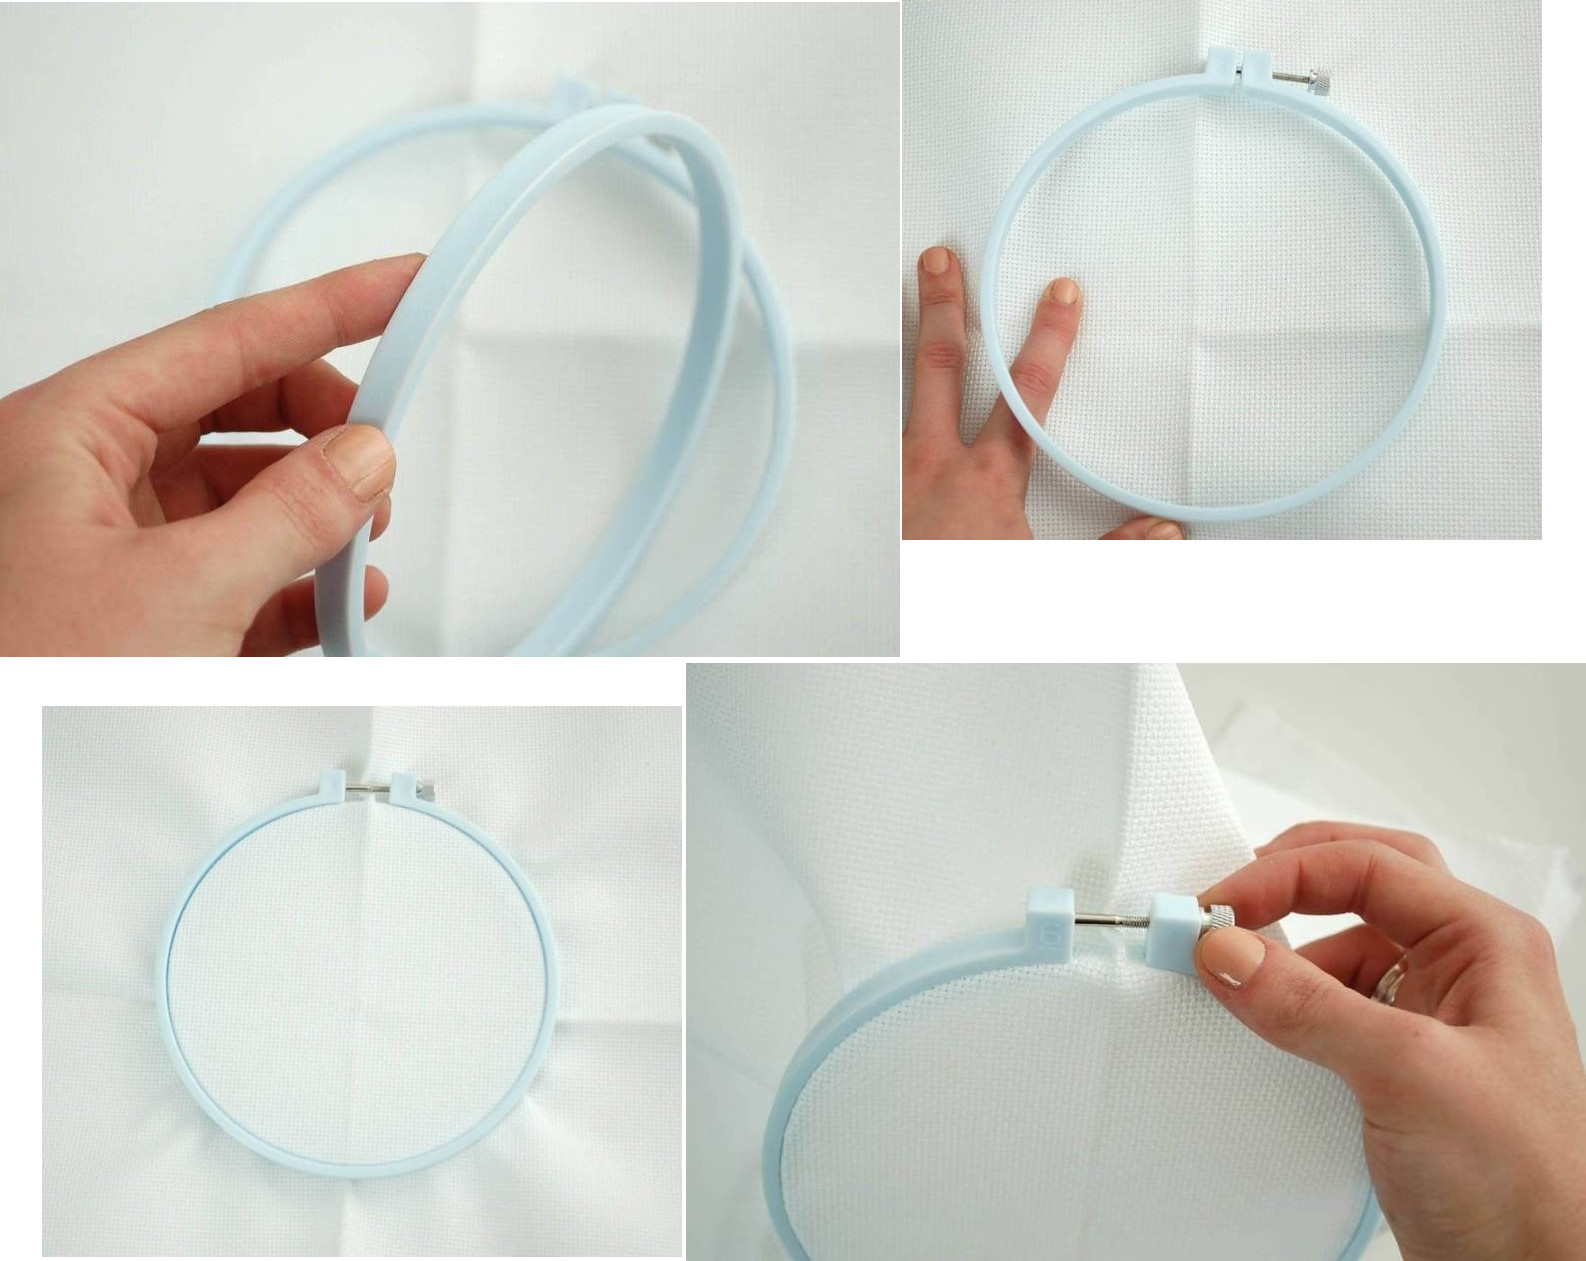
\includegraphics[width=4in]{InstallEmbroideryHoop.png}
\caption{Installing the Embroidery Hoop}
\label{fig:installembroideryhoop}
\end{centering}\end{figure}
To make sewing easier, we will be using an embroidery hoop.  An embroidery 
hoop will hold the fabric stiff and create a surface that is easy to stitch
on.  The embroidery hoop in in two pieces, the smaller loop goes underneath 
the fabric and the outer piece, which is adjustable, goes over the top and is 
tightened to hold the fabric securely.
\subsection{Wiring the GND wire}
We will start by running the ground wire.  This runs from the \texttt{GND} pad 
on the Gemma M0 to each if the \texttt{-} pads on the NeoPixels.
\begin{figure}[hbpt]\begin{centering}%
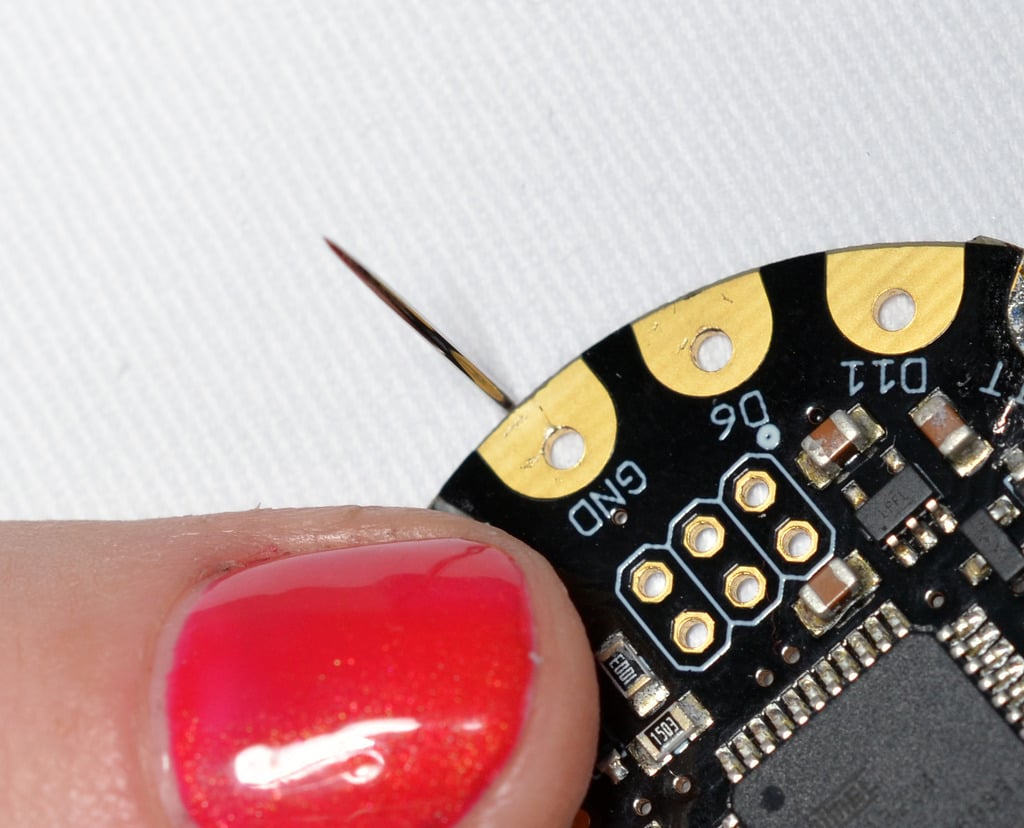
\includegraphics[height=2.75in]{flora_DSC_0099.png}
\caption{Bring up the needle near the \texttt{GND} pad}
\label{fig:flora_DSC_0099}
\end{centering}\end{figure}
\begin{figure}[hbpt]\begin{centering}%
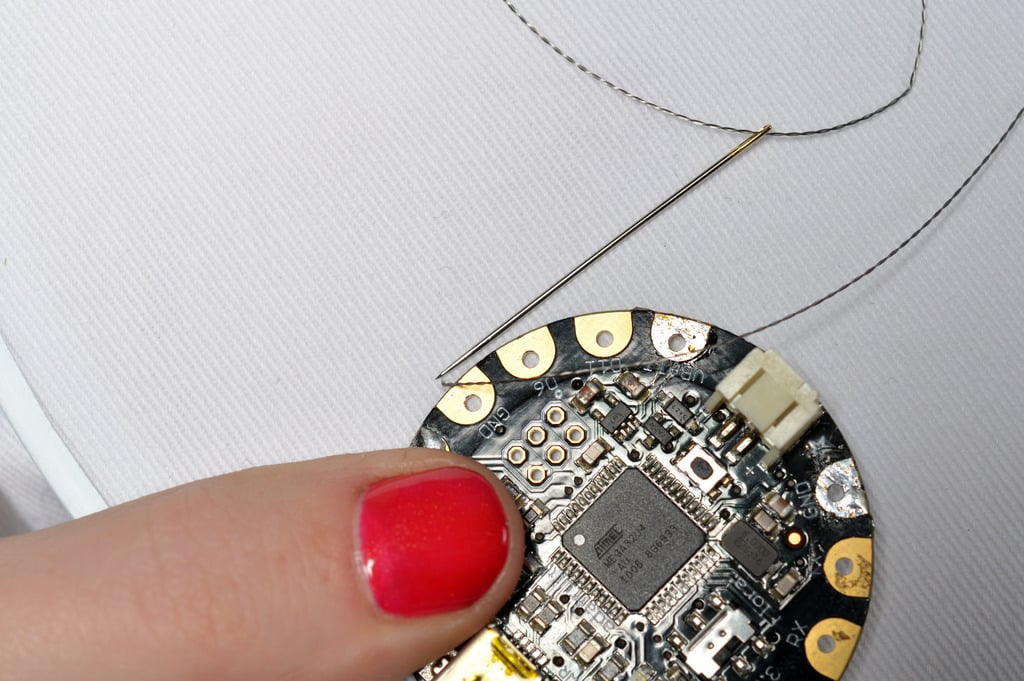
\includegraphics[height=2.75in]{flora_DSC_0100.png}
\caption{Pull though leaving about 5 inches behind the fabric}
\label{fig:flora_DSC_0100}
\end{centering}\end{figure}
\begin{figure}[hbpt]\begin{centering}%
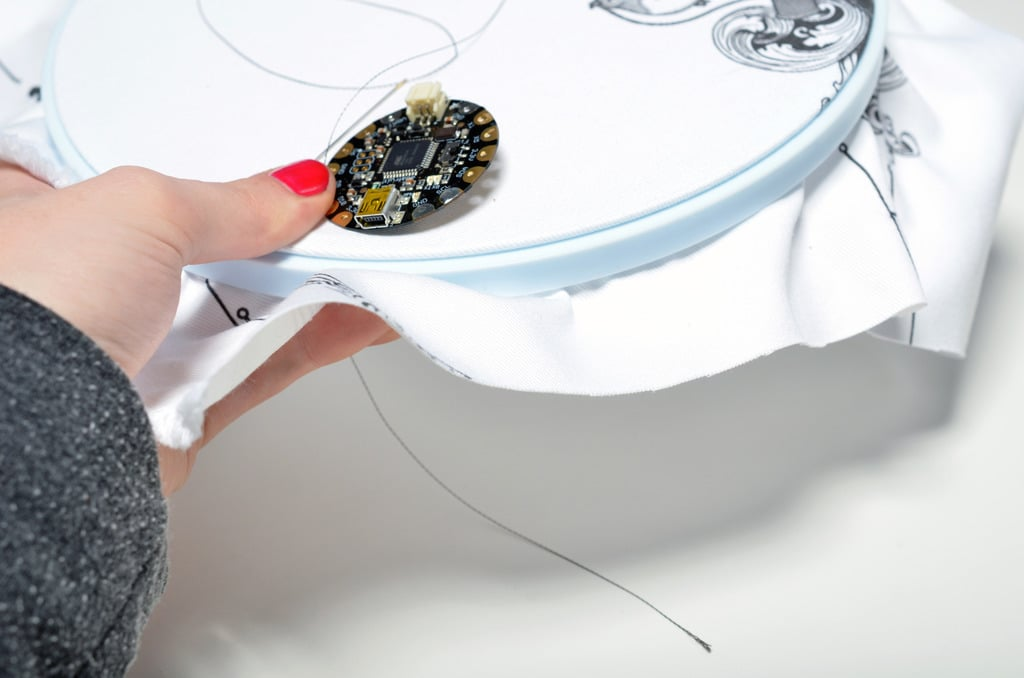
\includegraphics[height=2.75in]{flora_DSC_0101.png}
\caption{Leaving about 5 inches behind the fabric}
\label{fig:flora_DSC_0101}
\end{centering}\end{figure}
\begin{figure}[hbpt]\begin{centering}%
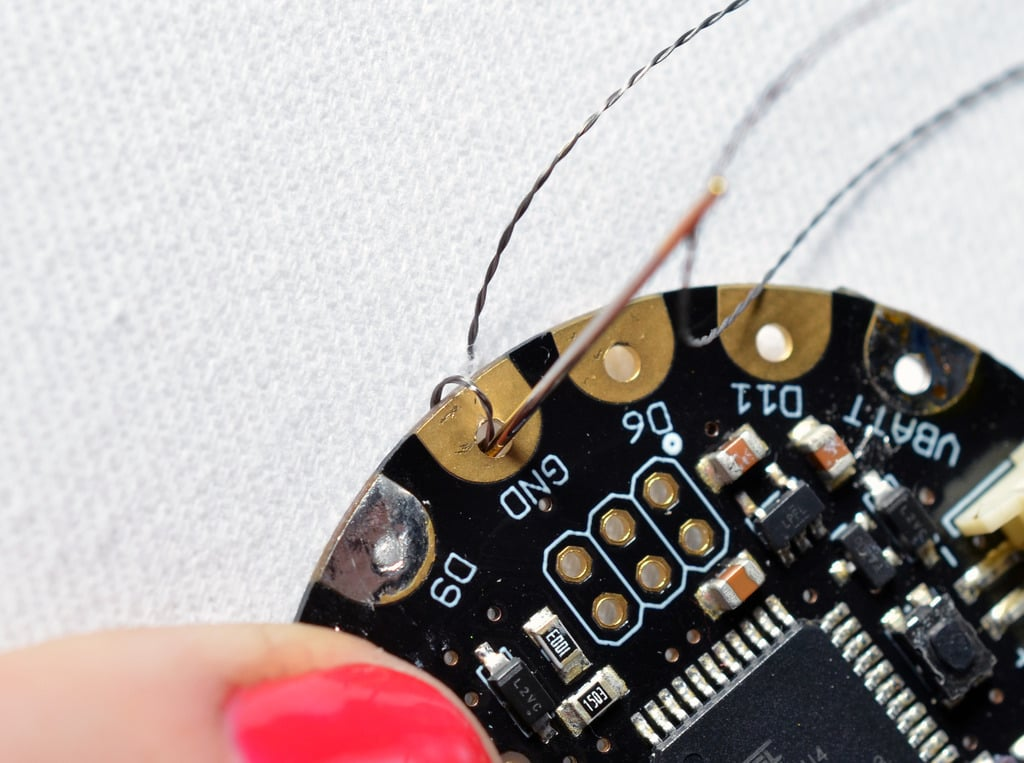
\includegraphics[height=2.75in]{flora_DSC_0103.png}
\caption{Wrap several times around the pad}
\label{fig:flora_DSC_0103}
\end{centering}\end{figure}
\begin{figure}[hbpt]\begin{centering}%
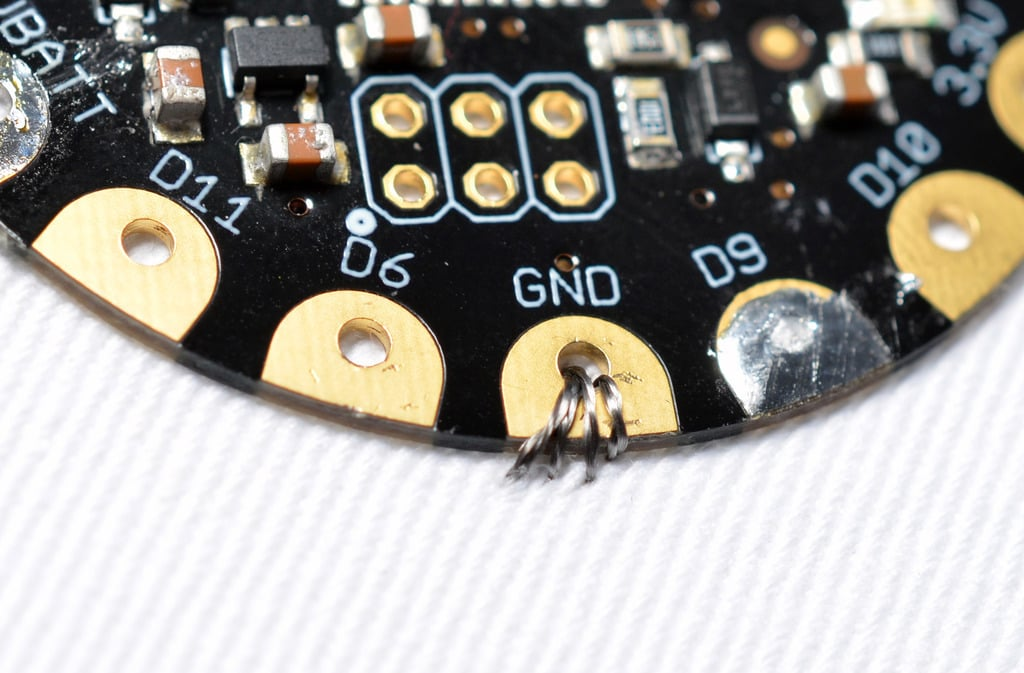
\includegraphics[height=2.75in]{flora_DSC_0105.png}
\caption{Wrap several tight loops around the pad}
\label{fig:flora_DSC_0105}
\end{centering}\end{figure}
\begin{figure}[hbpt]\begin{centering}%
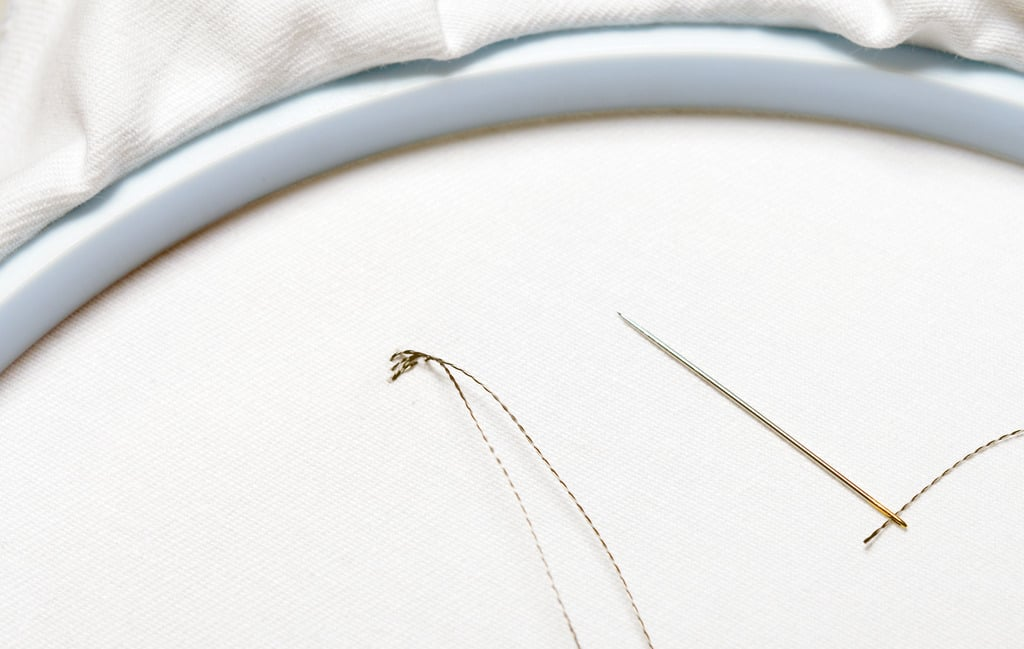
\includegraphics[height=2.75in]{flora_DSC_0106.png}
\caption{Ending on the back side near where you started}
\label{fig:flora_DSC_0106}
\end{centering}\end{figure}
\begin{figure}[hbpt]\begin{centering}%
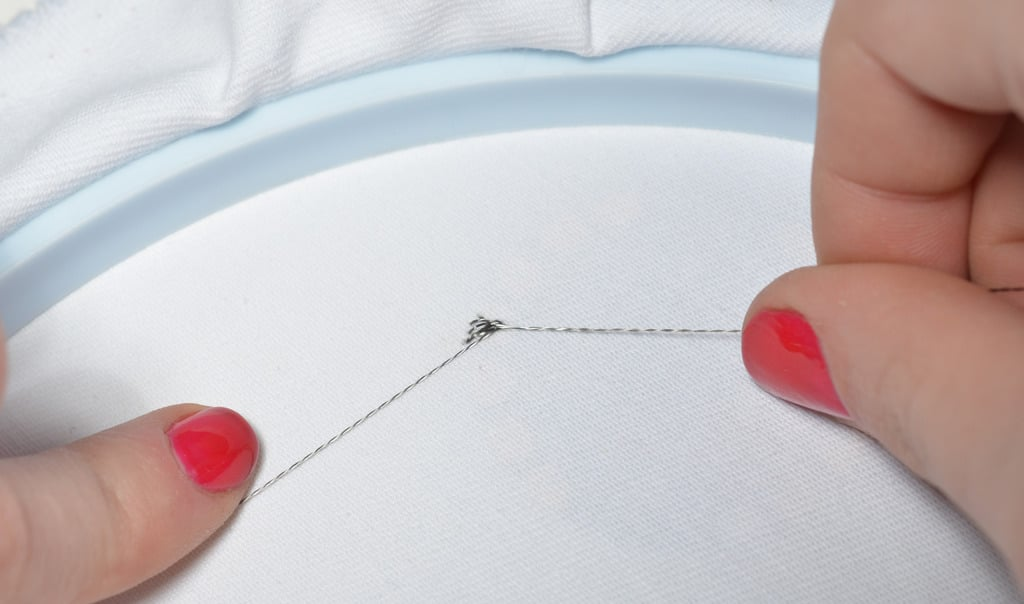
\includegraphics[height=2.75in]{flora_DSC_0107.png}
\caption{Tie a tight square knot}
\label{fig:flora_DSC_0107}
\end{centering}\end{figure}
\begin{figure}[hbpt]\begin{centering}%
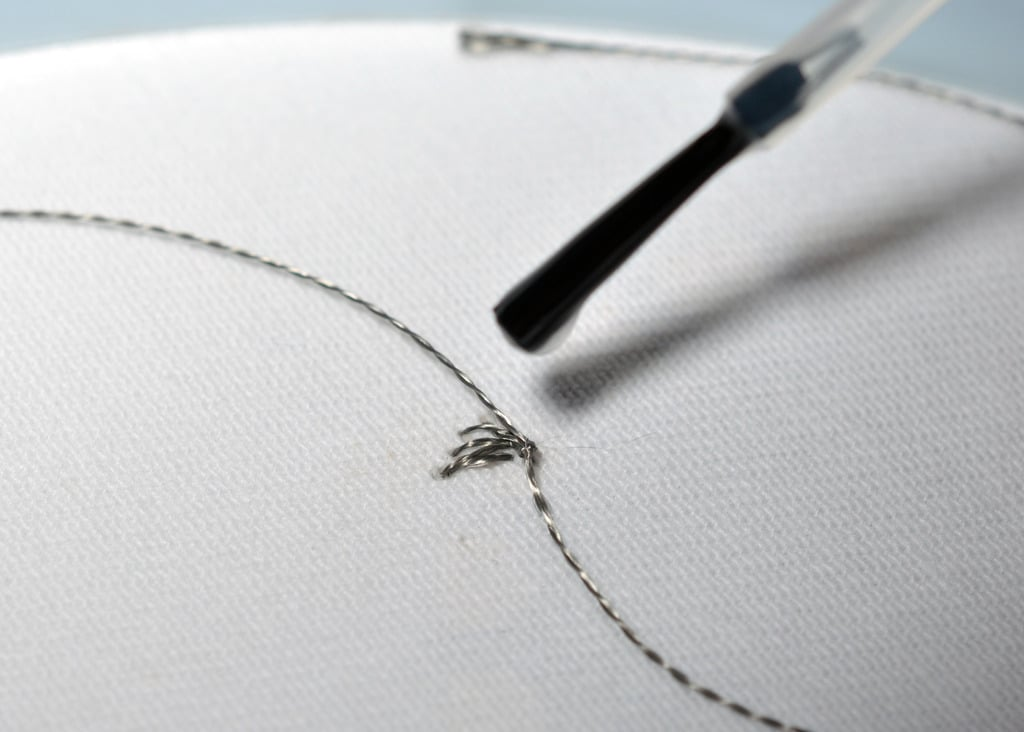
\includegraphics[height=2.75in]{flora_DSC_0109.png}
\caption{Apply a dab of nail polish to secure the knot}
\label{fig:flora_DSC_0109}
\end{centering}\end{figure}
\begin{figure}[hbpt]\begin{centering}%
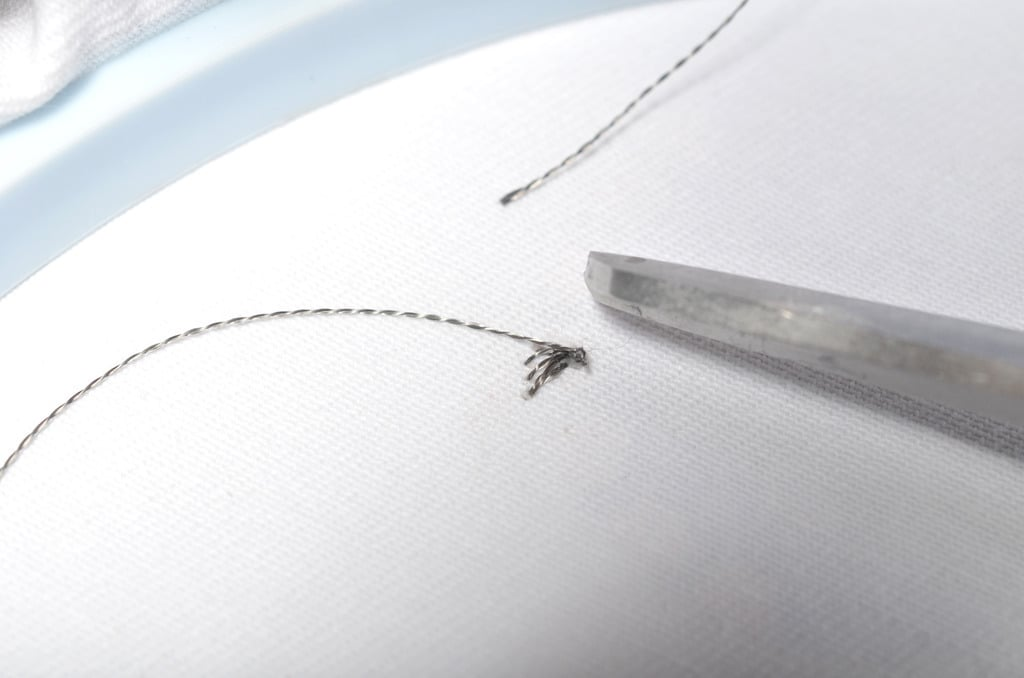
\includegraphics[height=2.75in]{flora_DSC_0111.png}
\caption{Trim the tail}
\label{fig:flora_DSC_0111}
\end{centering}\end{figure}
\begin{figure}[hbpt]\begin{centering}%
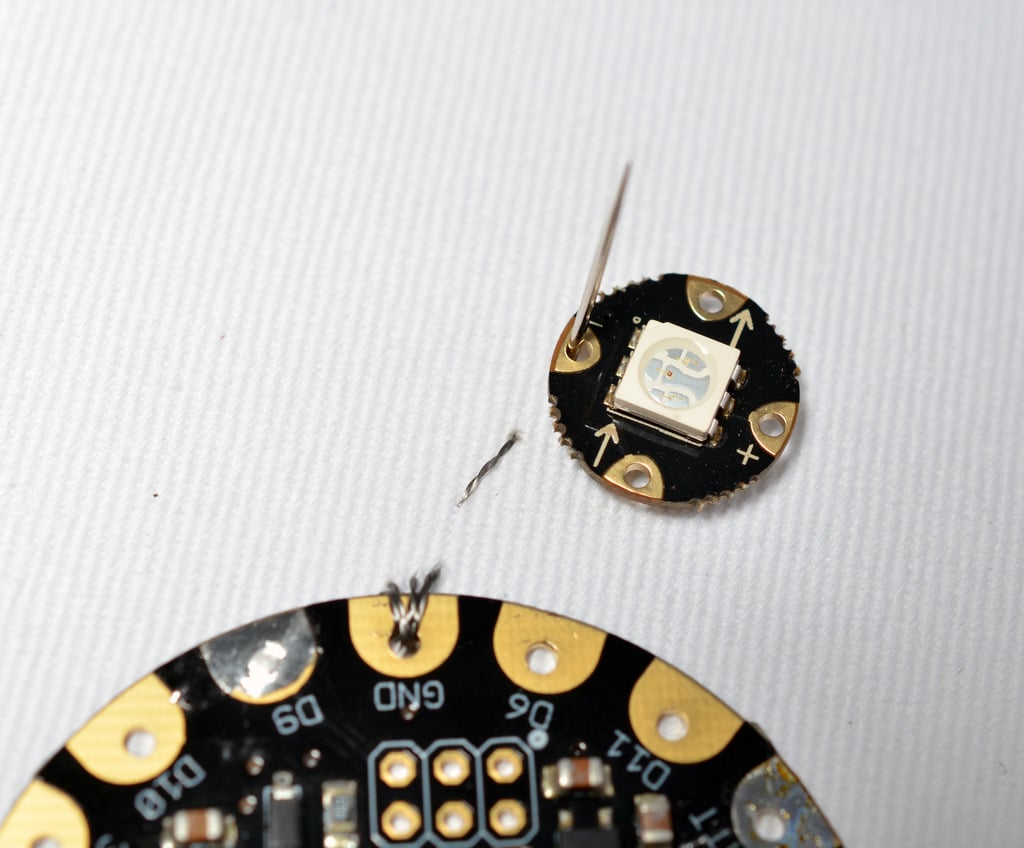
\includegraphics[height=2.75in]{flora_DSC_0113.png}
\caption{Use a running stitch to sew to the \texttt{-} pad of the first NeoPixel}
\label{fig:flora_DSC_0113}
\end{centering}\end{figure}
\begin{figure}[hbpt]\begin{centering}%
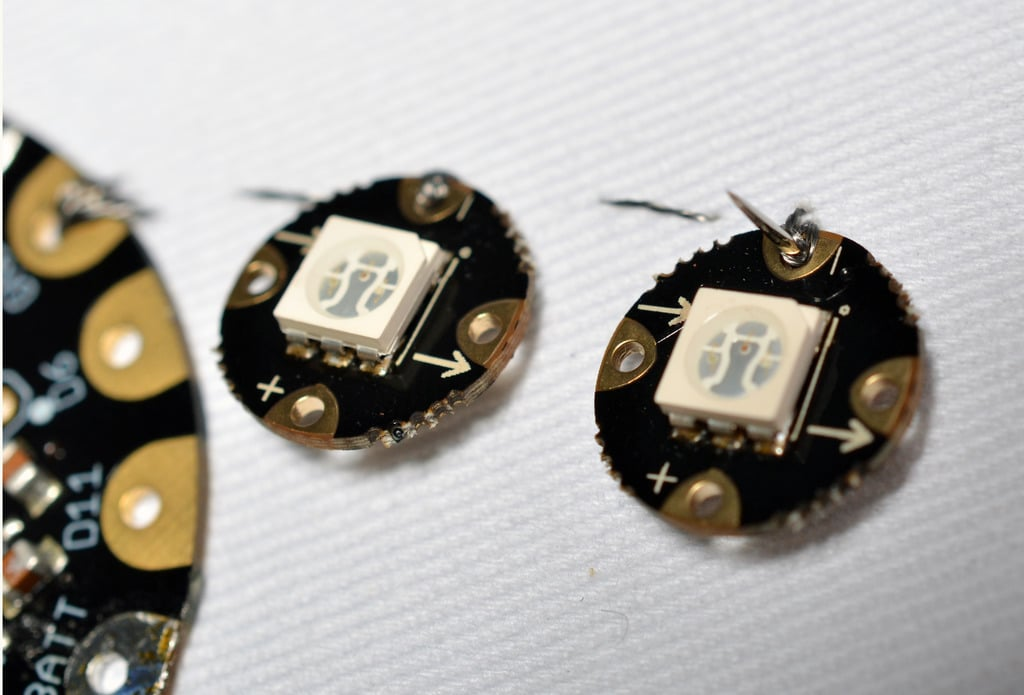
\includegraphics[height=2.75in]{flora_DSC_0115.png} 
\caption{Wrap several loops around the \texttt{-} pad and sew to the next NeoPixel}
\label{fig:flora_DSC_0115}
\end{centering}\end{figure}
\begin{figure}[hbpt]\begin{centering}%
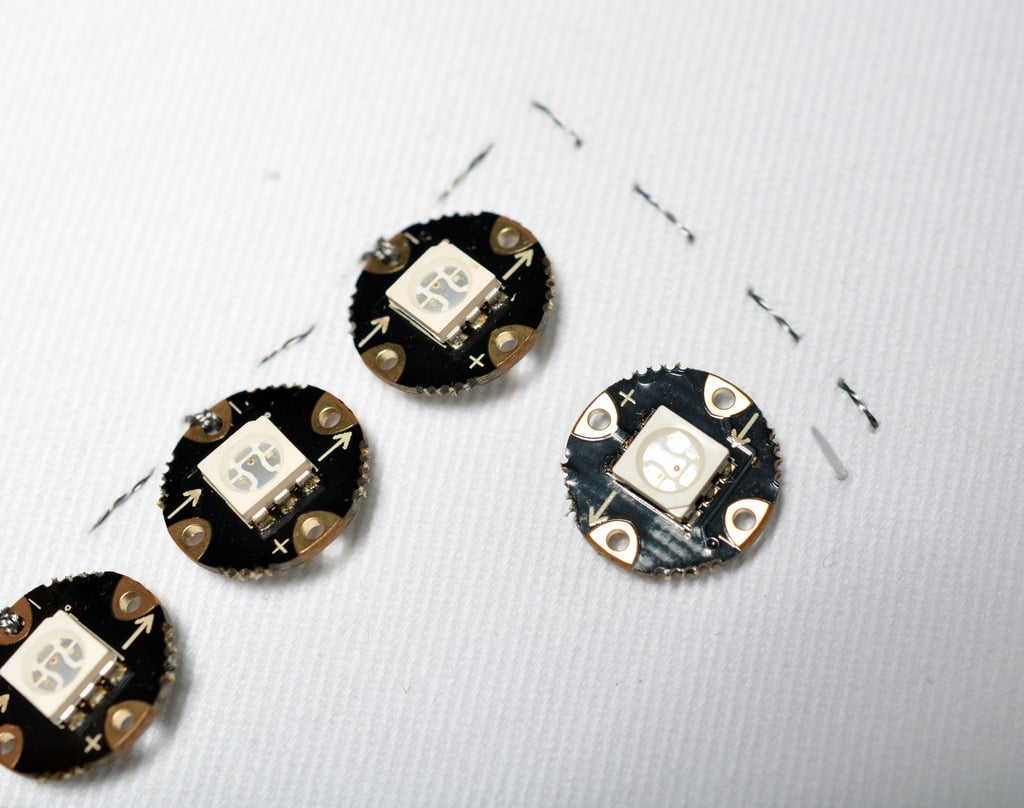
\includegraphics[height=2.75in]{flora_DSC_0116.png}
\caption{Continue to the next NeoPixel}
\label{fig:flora_DSC_0116}
\end{centering}\end{figure}
\begin{figure}[hbpt]\begin{centering}%
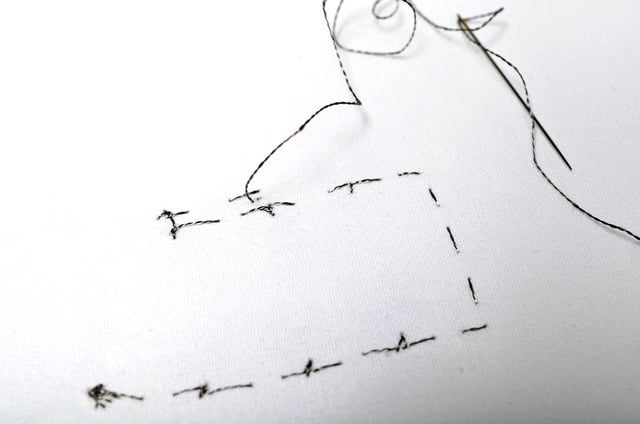
\includegraphics[height=2.75in]{flora_DSC_0118.png}
\caption{After the last NeoPixel, form a loop around the last stitch}
\label{fig:flora_DSC_0118}
\end{centering}\end{figure}
\begin{figure}[hbpt]\begin{centering}%
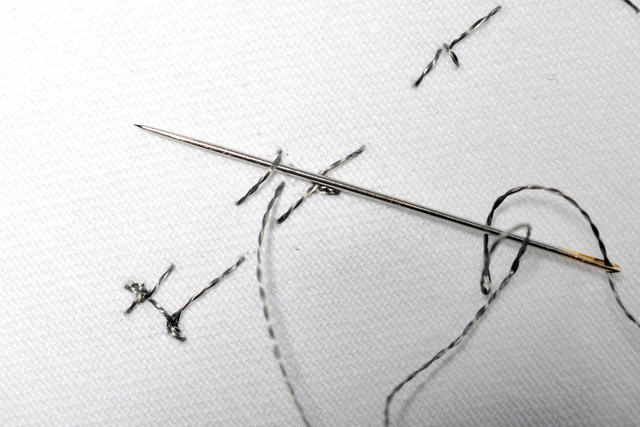
\includegraphics[height=2.75in]{flora_DSC_0119.png} 
\caption{And use that loop to start tieing a knot}
\label{fig:flora_DSC_0119}
\end{centering}\end{figure}
\begin{figure}[hbpt]\begin{centering}%
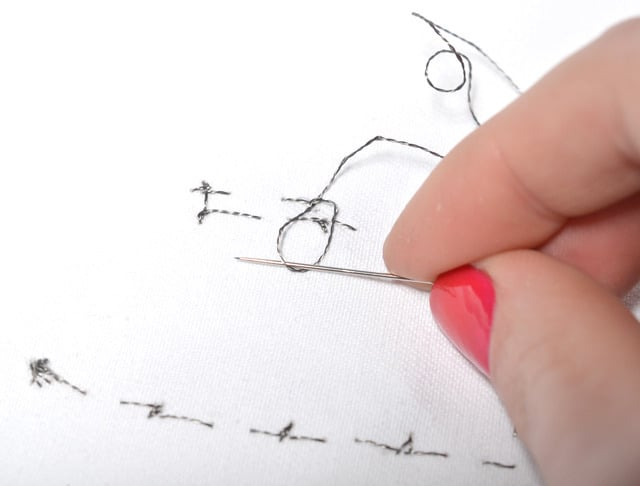
\includegraphics[height=2.75in]{flora_DSC_0120.png}
\caption{Tieing the knot}
\label{fig:flora_DSC_0120}
\end{centering}\end{figure}
\begin{figure}[hbpt]\begin{centering}%
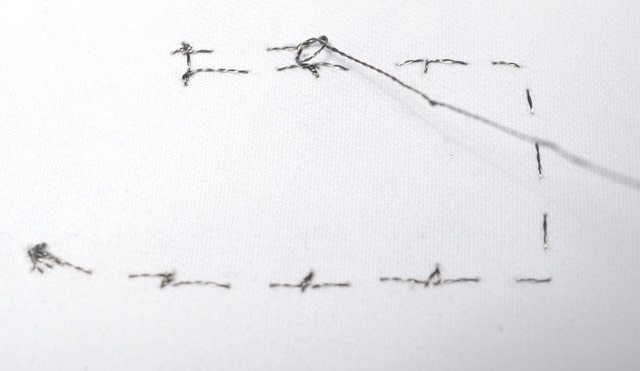
\includegraphics[height=2.75in]{flora_DSC_0121.png}
\caption{Tieing the knot}
\label{fig:flora_DSC_0121}
\end{centering}\end{figure}
\begin{figure}[hbpt]\begin{centering}%
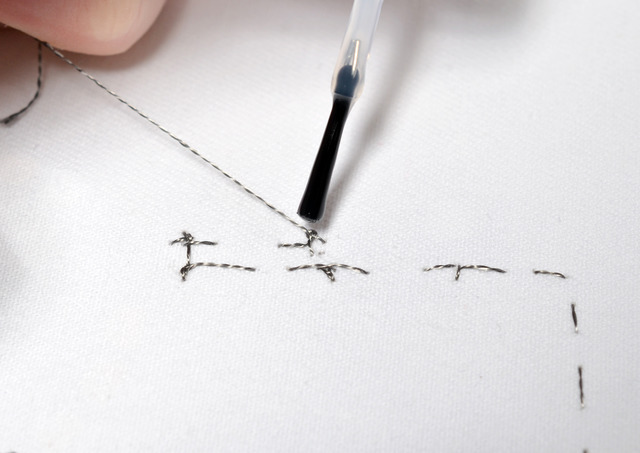
\includegraphics[height=2.75in]{flora_DSC_0123.png}
\caption{Secure the knot with nail polish}
\label{fig:flora_DSC_0123}
\end{centering}\end{figure}
\begin{figure}[hbpt]\begin{centering}%
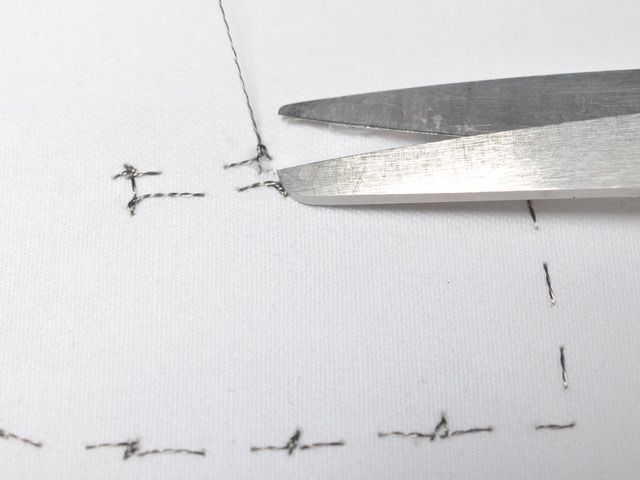
\includegraphics[height=2.75in]{flora_DSC_0125.png}
\caption{And trim the thread}
\label{fig:flora_DSC_0125}
\end{centering}\end{figure}
\clearpage
Repeat this process to stitch a ``wire'' from the \texttt{Vout} pad of the
Gemma M0 to the \texttt{+} pads of the NeoPixels. Then stitch a ``wire'' from
the \texttt{D1} pad to the in pointing arrow pad of the first NeoPixel, then
stitch a ``wire'' from the out pointing arrow pad of the first NeoPixel to the 
in pointing arrow pad of the second NeoPixel. Repeat for all of the NeoPixels. 
Nothing will be connected to the last NeoPixel's out pointing arrow pad.
\subsection{Snap Switch}
\begin{figure}[hbpt]\begin{centering}%
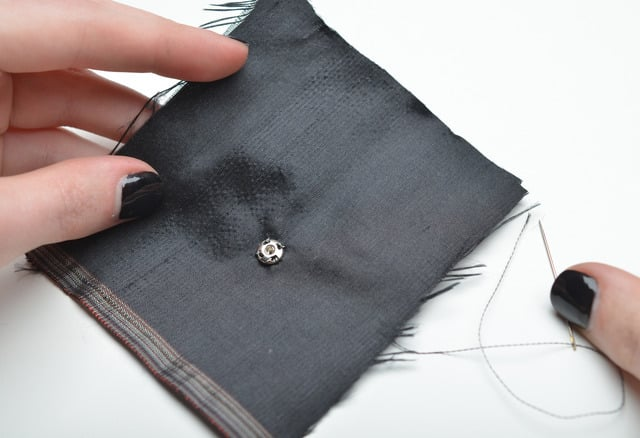
\includegraphics[height=2.75in]{flora-angler-embroidery-17.png}
\caption{Use conductive thread to sew one half of a snap to a scrap of fabric}
\label{fig:flora-angler-embroidery-17}
\end{centering}\end{figure}
\begin{figure}[hbpt]\begin{centering}%
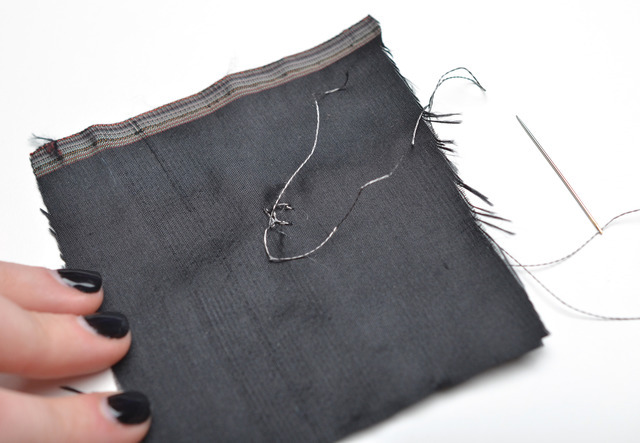
\includegraphics[height=2.75in]{flora-angler-embroidery-18.png}
\caption{Knot and seal the thread, leaving a long tail}
\label{fig:flora-angler-embroidery-18}
\end{centering}\end{figure}
\begin{figure}[hbpt]\begin{centering}%
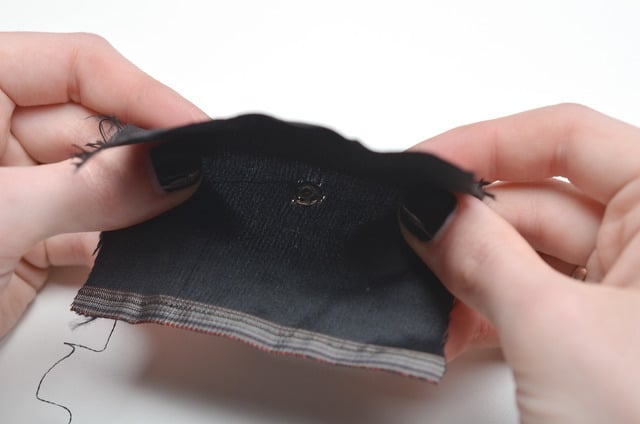
\includegraphics[height=2.75in]{flora-angler-embroidery-19.png}
\caption{Fold the scrap in half, with the snap inside}
\label{fig:flora-angler-embroidery-19}
\end{centering}\end{figure}
\begin{figure}[hbpt]\begin{centering}%
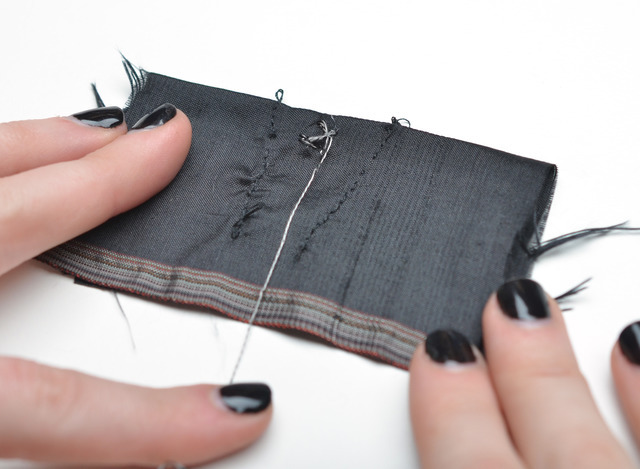
\includegraphics[height=2.75in]{flora-angler-embroidery-20.png}
\caption{Sew the sides to form a flap}
\label{fig:flora-angler-embroidery-20}
\end{centering}\end{figure}
\begin{figure}[hbpt]\begin{centering}%
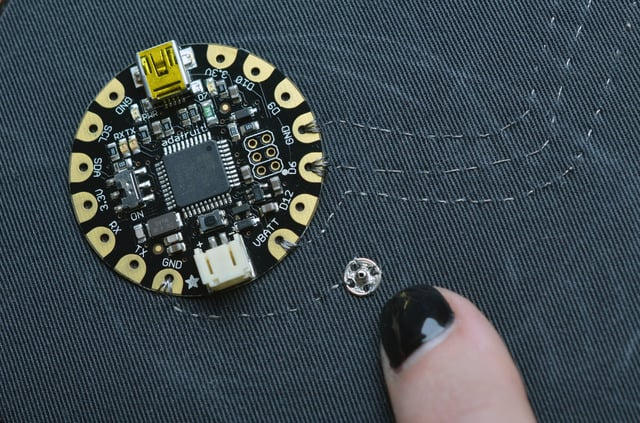
\includegraphics[height=2.75in]{flora-angler-embroidery-21a.png}
\caption{Sew the other half of the snap with conductive thread to the 
\texttt{GND} pad}
\label{fig:flora-angler-embroidery-21a}
\end{centering}\end{figure}
\begin{figure}[hbpt]\begin{centering}%
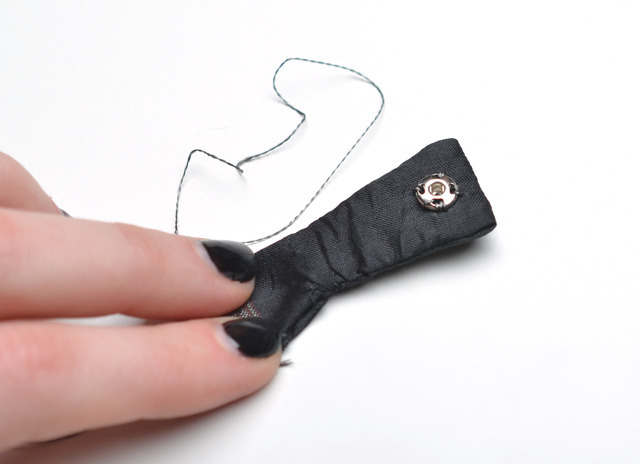
\includegraphics[height=2.75in]{flora-angler-embroidery-21.png}
\caption{Trim the scrap and turn right side out}
\label{fig:flora-angler-embroidery-21}
\end{centering}\end{figure}
\begin{figure}[hbpt]\begin{centering}%
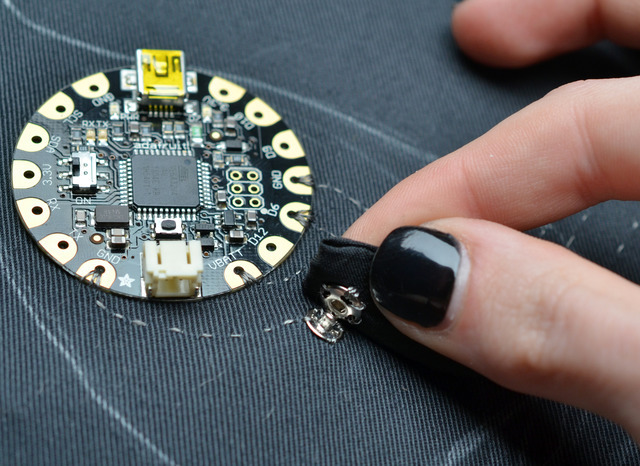
\includegraphics[height=2.75in]{flora-angler-embroidery-22.png}
\caption{Position the snap half on the flap with the half on the piece}
\label{fig:flora-angler-embroidery-22}
\end{centering}\end{figure}
\begin{figure}[hbpt]\begin{centering}%
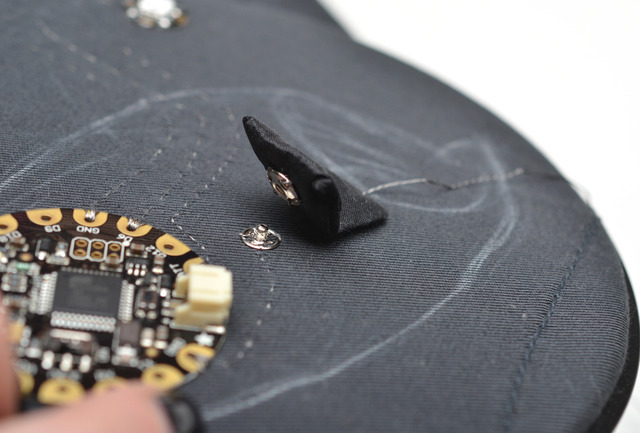
\includegraphics[height=2.75in]{flora-angler-embroidery-23.png}
\caption{Use regular thread to secure the flap}
\label{fig:flora-angler-embroidery-23}
\end{centering}\end{figure}
\begin{figure}[hbpt]\begin{centering}%
\includegraphics[height=2.75in]{flora-angler-embroidery-24.png}
\caption{Sew the tail of conductive thread from the flap to the \texttt{D2} pad}
\label{fig:flora-angler-embroidery-24}
\end{centering}\end{figure}
\clearpage
\part{Writing the CircuitPython code}
\lstinputlisting[numbers=left,caption={Python Code For Railroad Crossing Shirt}]{RailroadCrossing.py}
This is the code for my Railroad Crossing Shirt, which uses two NeoPixels for 
the crossing lights.  When the train embroidered flap is up and snapped in 
place, the NeoPixels alternatively blink in red, just like the lights at a 
railroad crossing.  When the flap is unsnapped and down the lights stay off.
\section{Description of the code}

The code is broken up into sections, with a blank line between each section.
Each section starts with a comment line. This is a line starting with a hash
character (\texttt{\#}). These lines are ignored by the Python processor -- they
are meant for people reading the code to get a better understanding of what
the code is meant to do.

The first part of the code (lines 1-5) load in library code, specificly:
\begin{enumerate}
\item The \texttt{board} module defines constants relating to the specific 
board.
\item The \texttt{digitalio} module defines classes, functions, and constants 
relating to basic digital I/O functions.
\item The \texttt{neopixel} module defines classes, functions, and constants 
supporting the use of NeoPixels.
\item The \texttt{time} module defines classes, functions, and constants 
providing time related functions.
\end{enumerate}

The next section, lines 7-10, define the NeoPixel strip: two NeoPixels using 
\texttt{D1} as the data line.

Then comes the code, lines 12-16, that defines the snap switch on \texttt{D2}.

Next, in lines 18-19 the LitPixel variable is initialized to zero. This
variable will tell us which NepPixel to light up each time through the main
loop.

Finally, in lines 21-35 is the main loop. This is a ``forever'' loop, since
\texttt{True} is always true. The code in the body of the loop, lines 23-35
are executed repeatedly so long as power is applied.

The loop body starts by turning all of the pixels in the pixel buffer off
(line 24). Then the snap switch is tested, if the snap switch is closed
(tested in line 26). If the switch is closed, the pixel indexed as
\texttt{LitPixel} is set to full red, then the \texttt{LitPixel} is switched
to the other pixel. One is added and the modulus (the remainder) of the number
of pixels (\texttt{NUMPIXELS}) is computed, in line 31. Then whether the
pixel was set or not, the pixel buffer is sent to the pixels, in line 33, 
Finally the program ``sleeps'' for 1 second (line 35).

\part{Installing the Battery}
\begin{figure}[hbpt]\begin{centering}%
\includegraphics[height=2.75in]{flora-angler-embroidery-28.png}
\caption{Cut a small hole next to the battery connector and feed the extension 
up and into the connector}
\label{fig:flora-angler-embroidery-28}
\end{centering}\end{figure}
\begin{figure}[hbpt]\begin{centering}%
\includegraphics[height=2.75in]{flora-angler-embroidery-29.png}
\caption{Route the cable to the pocket or pouch where the battery will be carried}
\label{fig:flora-angler-embroidery-29}
\end{centering}\end{figure}
The battery holder will be in one of pockets of the garment\footnote{If the
garment does not have pockets, a pocket or pouch can be added using a scrap of
fabric.}. We will be using the extension cable to make it possible to not need 
the Gemma M0 board to be right next to the pocket.
\begin{figure}[hbpt]\begin{centering}%
\includegraphics[height=2.75in]{flora-angler-embroidery-30.png}
\caption{Make a small hole in the pocket or pouch for the other end of the cable}
\label{fig:flora-angler-embroidery-30}
\end{centering}\end{figure}
\begin{figure}[hbpt]\begin{centering}%
\includegraphics[height=2.75in]{flora-angler-embroidery-31.png}
\caption{Draw the cable though the hole to make it available for connecting 
the battery holder}
\label{fig:flora-angler-embroidery-31}
\end{centering}\end{figure}
\begin{figure}[hbpt]\begin{centering}%
\includegraphics[height=2.75in]{flora-angler-embroidery-32.png}
\caption{Secure the cable to the inner side of the garment with a few whip stitches}
\label{fig:flora-angler-embroidery-32}
\end{centering}\end{figure}
\begin{figure}[hbpt]\begin{centering}%
\includegraphics[height=2.75in]{flora-angler-embroidery-33.png}
\caption{Use whip stitches multiple places along the length of the cable to 
secure it}
\label{fig:flora-angler-embroidery-33}
\end{centering}\end{figure}
\begin{figure}[hbpt]\begin{centering}%
\includegraphics[height=2.75in]{flora-angler-embroidery-35.png}
\caption{Use whip stitches multiple places along the length of the cable to 
secure it}
\label{fig:flora-angler-embroidery-35}
\end{centering}\end{figure}
\end{document}
